
\documentclass[authoryear]{elsarticle}

\usepackage[utf8]{inputenc}
\usepackage[english,russian]{babel}

\usepackage{amsmath}
\usepackage{bm}
\usepackage{tikz}
\usepackage{pgfplots}
\usepackage{color, colortbl}
\usepackage{graphicx}

\graphicspath{{pictures/}}

\usepackage{hyperref}

\newtheorem{thm}{Theorem}
\newtheorem{lem}[thm]{Lemma}
\newproof{pf}{Proof}

\journal{Annals of Nuclear Energy}

\bibliographystyle{elsarticle-harv}

\begin{document}

\begin{frontmatter}

\title{State change modal method для численного моделирования of dynamic processes in a nuclear reactor}

\author[ki]{Alexander V. Avvakumov}
\ead{Avvakumov2009@rambler.ru}

\author[nsi]{Valery~F.~Strizhov}
\ead{vfs@ibrae.ac.ru}

\author[nsi,univ]{Petr N. Vabishchevich\corref{cor}}
\ead{vabishchevich@gmail.com}

\author[univ]{Alexander O. Vasilev}
\ead{haska87@gmail.com}

\address[ki]{National Research Center \emph{Kurchatov Institute},  1, Sq. Academician Kurchatov, Moscow, Russia}
\address[nsi]{Nuclear Safety Institute, Russian Academy of Sciences, 52, B. Tulskaya, Moscow, Russia}
\address[univ]{North-Eastern Federal University, 58, Belinskogo, Yakutsk, Russia}

\cortext[cor]{Corresponding author}

\begin{abstract}
Моделирование динамических процессов в ядерных реакторах проводится, 
чаще всего, на основе описания нейтронного потока в многогрупповом диффузионном приближении. 
Базовая модель включает многомерную систему связанных уравнений параболического типа и обыкновенных дифференциальных уравнений. 
Динамические процессы моделируются последовательной сменой состояний реактора, которые характеризуются заданными 
постоянными коэффициентами уравнений.
В modal method приближенное решение представляется в виде разложения по первым собственным функциям 
некоторой спектральной задачи. Численно-аналитический метод основан на использовании of dominant time-eigenvalues of
a nuclear reactor для  многогрупповой диффузионной модели с учетом запаздывающих нейтронов.
Проведено численное моделирование нестационарного процесса в рамках 
двухгруппового приближения для тестовой модели реактора на тепловых нейтронах VVER-1000,
которая характеризуется тем, что часть собственных значений является комплексными.
\end{abstract}

\begin{keyword}
Neutron diffusion equations \sep  multi-group approximation \sep space-time kinetic 
\sep spectral problem \sep modal method.

\end{keyword}

\end{frontmatter}


\section{Introduction} 

Среди основных физических процессов, происходящих в ядерном реакторе \citep{duderstadt1976nuclear}, 
основное внимание уделяется переносу нейтронов. 
Для их описания привлекается достаточно сложное интегро-дифференциальное уравнение, 
в котором распределение потока нейтронов зависит от времени, энергии, пространственных 
и угловых переменных \citep{hetrick1971dynamics,stacey}. 
Практические расчеты ядерных реакторов, как правило, проводятся с использованием 
более простых систем уравнений многогруппового диффузионного приближения \citep{marchuk1986numerical,lewis1993computational,sutton1996diffusion,cho2005fundamentals}.
В настоящее время diffusion models are derived 
and applied using sophisticated homogenization methodologies (see \cite{sanchez2009assembly,dugan2016cross}) 
which define parameters of the multigroup diffusion equations that enable one to take into account transport effects. 

Расчетная модель представляет собой систему связанных параболических уравнений второго порядка, которая
при учете запаздывающих нейтронов дополняется системой обыкновенных дифференциальных уравнений.
Инженерные нейтронно-физические коды, которые предназначены для моделирования переноса нейтронов в диффузионном групповом приближении,
базируются, чаще всего, на конечно-разностных аппроксимациях по пространству. 
Для повышения точности расчета широкое применение нашли нодальные методы 
(см., например, \cite{smith1979analytic,lawrence1986progress}), 
которые позволяют проводить расчеты на достаточно грубой сетке (несколько точек на тепловыделяющую сборку в плане и несколько десятков слоев по высоте). В основе нодальных методов лежит представление нейтронного потока в пределах расчетного элемента в виде полинома малой степени или набора функций по одной из координат (или на плоскости). 
Нодальные методы в ряде случаев можно связать \citep{grossman2007nodal} со специальными вариантами конечно-элементной аппроксимации.
Следует отметить, что более уместно использование стандартных процедур повышения точности конечно-элементного приближения при приближенном
решении краевых задач, связанное со сгущение расчетной сетки и использовании конечных элементов более высокой степени.
Такая технология используется в \cite{vidal2014solution,avvakumov2017spectral} 
при рассмотрении спектральных задач для the multigroup diffusion equations.

При моделировании динамики нейтронно-физических процессов используются стандартные методы приближенного решения нестационарных
задач \citep{sutton1996diffusion,cho2005fundamentals,stacey}. Наибольшее внимание уделяется двухслойным схемам с весами ($\theta$-метод, схема с весами) \citep{Ascher2008,LeVeque2007,HundsdorferVerwer2003},
используются схемы Рунге-Кутта, схемы Розенброка \citep{Butcher2008,HairerWanner2010}.
Для характеристики динамической природы реактора используется 
спектральный параметр $\alpha$. Он определяется как главное собственное
значение 
спектральной задачи (time-eigenvalue, $\alpha$-eigenvalue problem), которая связывается с нестационарными уравнениями диффузии нейтронов
\citep{Bell1970,modak2007scheme,verdu20103d}.
По аналогии с обычными задачами теплопроводности (смотри, например, \cite{luikov2012analytical,samarskii1996computational}) мы можем выделить регулярный режим
реактора. При больших временах поведение нейтронного поля носит асимптотический характер, когда можно
говорить о пространственно-временной факторизации решения,
амплитуда которого есть $\exp(-\alpha t)$, форм-функция --- собственная функция спектральной задачи. 
Для моделирования регулярного режима реактора необходимо ориентироваться на использование чисто неявных схем, 
в то время, как схема Кранка-Николсон является непригодной \citep{nd-mm}.

Нейтронно-физические расчеты реальных трехмерных конструкций требуют использования больших расчетных сеток,
динамические процессы моделируются на больших временах. В силу сложности математической модели,
применения больших расчетных сеток мы должны использовать современные многопроцессорные вычислительные системы.
Параллельные вычислительные алгоритмы базируются на переходе  к последовательности решения более простых
задач для отдельных процессов. Успех достигается применением decoupling технологии (расщепления по физических процессам
\citep{Vabishchevich2014}), декомпозиции расчетной области на подобласти \citep{ToselliWidlund2005},
итерационных методов решения систем алгебраических уравнений \citep{Saad2003}. 
Применительно к спектральным задачам for the neutron diffusion problem  
domain decomposition methods используются, например, в \cite{guerin2010domain}. 
Особенности решения нестационарных задач на параллельных компьютерах 
учитываются построением специальных итерационных методов типа the parareal in time algorithm \citep{maday2005parareal}. 
В работе \cite{baudron2014parareal} такой подход реализован при численном решении нестационарных multigroup neutron kinetics
equations involving a time delayed contributions.

В теории и практике нейтронно-физических расчетов большое внимание уделяется
быстрым методам построения приближенных решений. В этой связи отметим
класс методов для моделирования нестационарного 
переноса нейтронов в диффузионном групповом приближении,
который связан с мультипликативным представлением решения --- space-time factorization methods) и квазистатический метод 
(quasistatic method)  \citep{dodds1976accuracy,chou1990three,goluoglu2001time,dulla2008quasi,dahmani20013d}.
В этом случае приближенное решение ищется в виде произведения двух функций: одна из которых зависит от времени и связывается с амплитудой,
вторая (shape function) --- описывает пространственное распределение.  
The shape function часто связывается с fundamental собственной функцией тех или иных 
задач на собственные значения для  neutron diffusion equations.

При использовании quasistatic method задача максимально упрощается, но рассчитывать на хорошую точность приближенного решения
не приходиться, в частности, при расчете 
динамических режимов со сложной перестройкой поля плотности нейтронного потока.
В силу этого давно и успешно развивается более общий подход --- the modal method  \citep{stacey1967modal,stacey1969space,sutton1996diffusion}.
В этом случае решение ищется в виде суммы нескольких доминантных собственных значений с коэффициентами,
которые зависят от времени.

To characterize the reactor dynamic processes привлекаются some spectral
problems \citep{Bell1970,hetrick1971dynamics,stewart1976spectral,stacey}.
The processes occurring in a nuclear reactor are essentially non-stationary. 
The stationary state of neutron flux is characterised by local balancing of neutron absorption and and generation
and is usually described by solution of a spectral problem (Lambda modes problem, $\lambda$-eigenvalue problem).
The fundamental eigenvalue (maximal eigenvalue) is called $k$-effective of the reactor core.
The nodal method на основе использования решения $\lambda$-eigenvalue problem обсуждаются, например,
в работах \cite{verdu1998modal,miro2002nodal,gonzalez2009high}. В частности, отдельного внимания заслуживают вопросы решения
связанной системы уравнений для нестационарных коэффициентов разложения. 

Нестационарные процессы естественно описывать на основе разложения 
приближенного решения по собственным функциям 
time-eigenvalue, $\alpha$-eigenvalue problem \citep{ginestar2002transient,verdu20103d,verdu2014modal}.
В более простой модели без учета запаздывающих нейтронов modal methods
используется в работе \cite{modak2007scheme}.
Принципиальный момент связан с тем, что при таком подходе мы имеем несвязанную систему уравнений для коэффициентов.
Необходимо также отметить, что как при использовании  $\lambda$-eigenvalue problem, так и при использовании
$\alpha$-eigenvalue problem мы имеем, вообще говоря, комплексные собственные значения.
Для задания начального состояния это приводит к необходимости решения соответствующих adjoint spectral problems.

В настоящей работе формулируется общая стратегия приближенного решения нестационарных задач нейтроники ядерных реакторов,
которая ориентирована на быстрые расчеты реального времени --- State Change Modal (SCM) метод.
Динамическое поведение ядерного реактора рассматривается как последовательность его состояний, каждое из которых
характеризуется своим набором постоянных коэффициентов системы  the multigroup diffusion equations.
Считается, что переход из одного состояния в другое происходит мгновенно.
Нейтронное поле отдельного состояния рассчитывается на основе использования modal method ---
представление решения задачи в виде разложения по доминантным собственным функциям $\alpha$-eigenvalue problem
с учетом запаздывающих нейтронов (the full Alpha method). 
Real-time вычисления обеспечиваются тем, что необходимый набор собственных значений и собственных функций
детерминистического состояния реактора рассчитываются заранее.

The paper is organised as follows. 
Динамическая модель ядерного реактора на основе системы the multigroup diffusion equations is given in Section 2. 
Общая стратегия численного  моделирования нестационарных процессов на основе SCM метода 
описываются in Section 3. 
Ключевые  вычислительные  аспекты SCM технологии are discussed in Section 4.
Two-dimensional test problems  for VVER-1000 reactor is discussed in Section 5. 
Проведено моделирование динамического процесса, который соответствует 
двум состояниям (надкритическому и подкритическому) реактора: переход с регулярного режима накритического состояния 
на подкритическое состояние реактора.
The results of the work are summarised in Section 6.

\section{Problem statement}

The neutron flux  моделируется in multigroup diffusion approximation. The neutron dynamics is considered in the bounded convex two-dimensional or three-dimensional area  $\Omega$ ($\bm x = \{x_1, ..., x_d\} \in \Omega, \ d = 2,3$) with boundary $\partial \Omega$. The neutron transport is described by the system of equations:
\begin{equation}\label{1}
\begin{split}
 \frac{1}{v_g} \frac{\partial \phi_g}{\partial t} - & \nabla \cdot D_g \nabla \phi_g + \Sigma_{rg} \phi_g 
 - \sum_{g\neq g'=1}^{G} \Sigma_{s,g'\rightarrow g} \phi_{g'} \\
 =  & \ (1-\beta) \chi_g \sum_{g'=1}^{G} \nu \Sigma_{fg'} \phi_{g'} + \widetilde{\chi}_g \sum_{m=1}^{M} \lambda_m c_m , \quad 
 g = 1,2, ..., G .
\end{split}
\end{equation} 
Here $\phi_g(\bm x,t)$ --- neutron flux of $g$ group at point $\bm x$ and time $t$,
$G$ --- number of energy groups,
$v_g$ --- effective velocity of neutrons in the group $g$,
$D_g(\bm x)$ --- diffusion coefficient, $\Sigma_{rg}(\bm x,t)$ --- removal cross-section,
$\Sigma_{s,g'\rightarrow g}(\bm x,t)$ --- scattering cross-section from group $g'$ to group $g$,
$\beta$ --- effective fraction of delayed neutrons, $\chi_g$, $\widetilde{\chi}_g$  --- spectra of prompt and delayed neutrons, 
$\nu\Sigma_{fg}(\bm x,t)$ --- generation cross-section of group $g$,
$c_m$ --- density of sources of delayed neutrons of $m$-type,  $\lambda_m$ --- decay constant of sources of delayed neutrons,
$M$ --- number of types of delayed neutrons.
The density of sources of delayed neutrons is described by the equations:
\begin{equation}\label{2}
 \frac{\partial c_m}{\partial t} + \lambda_m c_m = \beta_m \sum_{g=1}^{G} \nu \Sigma_{fg} \phi_g ,
 \quad m = 1,2, ..., M , 
\end{equation} 
where $\beta_m$ is a fraction of delayed neutrons of $m$-type, and
\[
 \beta = \sum_{m=1}^{M} \beta_m .
\] 
System of equations (\ref{1}), (\ref{2}) is supplemented with corresponding initial and boundary conditions.

The albedo-type conditions are set at the boundary $\partial \Omega$ of the area $\Omega$:
\begin{equation}\label{3}
 D_g\frac{\partial \phi_g}{\partial n} + \gamma_g \phi_g = 0, \quad 
 \quad g = 1,2, ..., G ,
\end{equation}
where $n$ --- outer normal to the boundary $\partial \Omega$.
Начальное состояние определяется следующим образом:
\begin{equation}\label{4}
 \phi_g(\bm x,0) = \phi_g^0(\bm x), 
 \quad c_m(\bm x,0) = c_m^0(\bm x) . 
\end{equation} 

Let's write the boundary problem (\ref{1})--(\ref{4}) in operator form. The vectors 
 $\bm \phi = \{\phi_1, \phi_2, ..., \phi_G\}$, $\bm c = \{c_1, c_2, ..., c_M\}$ 
and matrices are defined as follows:
\[
\begin{align}
 V & = (v_{g g'}), &
  \quad v_{g g'} & = \delta_{g g'} v_g^{-1}, \\
 D & = (d_{g g'}), &
 \quad d_{g g'} & = - \delta_{g g'} \nabla \cdot D_g \nabla, \\
 S & = (s_{g g'}), &
 \quad  s_{g g'} & =  \delta_{g g'} \Sigma_g - \Sigma_{s,g'\rightarrow g}, \\
 R & = (r_{g g'}), &
 \quad  r_{g g'} & = (1-\beta)\chi_g \nu \Sigma_{fg'}, \\
 B & = (b_{g m}), &
 \quad b_{g m} & = \widetilde{\chi}_g \lambda_m, \\
 \Lambda & = (\lambda_{m m'}), &
 \quad  \lambda_{m m'} & = \lambda_m \delta_{m m'}, \\
 Q & = (q_{mg}), &
 \quad  q_{mg} & = \beta_m \nu \Sigma_{fg}, \\
 g, g' & = 1,2, ..., G, &
 \quad m, m'  &= 1,2, ....,M,  
\end{align}
\]
where
\[
 \delta_{g g'} = \left \{ 
 \begin{matrix}
 1, & g = g', \\
 0, & g \neq  g',
 \end{matrix}
 \right . 
\] 
is the Kronecker symbol.
We shall use the set of vectors $\bm \phi$, whose components 
satisfy the boundary conditions (\ref{3}). 
Using the set definitions, the system of equations (\ref{1}), (\ref{2})  
can be written in the form of first-order equation of evolution:
\begin{equation}\label{5}
\begin{split}
V(t) \frac{d \bm \phi}{d t} + (D(t)+S(t)) \bm \phi &= R(t) \bm \phi + B(t)\bm c,
\\
\frac{d \bm c}{d t} + \Lambda(t)\bm c &= Q(t) \bm \phi. 
\end{split}
\end{equation}  
Для уравнений (\ref{5})  рассматривается задача Коши, когда
\begin{equation}\label{6}
 \bm \phi(0) = \bm \phi^0,
 \quad   \bm c(0) = \bm c^0,
\end{equation} 
где  с учетом (\ref{4}) $\bm \phi^0 = \{ \phi_1^0,  \phi_2^0, ...,  \phi_G^0 \}$,  $\bm c^0 = \{c_1^0, c_2^0, ..., c_M^0\}$.

Для приближенного решения задачи Коши (\ref{5}), (\ref{6}) 
используется два основных подхода. Первый из них связан с использованием стандартных
двухслойных или трехслойнвх схем, которые широко используются при численном решении параболических задач \citep{Samarskiibook}.
Операторные матрицы $V, D$ диагональные, а $S$ -- нижняя треугольная матрица. 
Существенное связывание уравнений обусловлено только оператором генерации нейтронов $R$.
Актуальной является проблема выбора расчетных схем среди устойчивых разностных схем, 
которые	является оптимальными по тем или иным дополнительным критериям. 
В теории разностных схем выделен класс асимптотически устойчивых 
разностных схем, которые \citep{samarskii1996computational} обеспечивают правильное
поведение приближенного решения при больших временах. 
В теории численных методов решения систем обыкновенных дифференциальных
уравнений \citep{Butcher2008,Gear1971} введено понятие $L$-устойчивых методов,
в которых с несколько других позиций также отслеживается 
асимптотическое поведение приближенного решения
при больших временах. Чисто неявная схема имеет лучшие асимптотические свойства,
чем симметричная схема (схема Кранка-Николсон) (ses \cite{VabishchevichSM}), 
что важно при исследовании регулярного режима ядерного реактора \citep{nd-mm}.

Вторым классом являются численно-аналитические методы решения задачи (\ref{5}), (\ref{6}),
наиболее ярким примером которых выступают отмеченные выше modal methods  \citep{stacey1967modal,stacey1969space,sutton1996diffusion}.
Они учитывают линейную природу рассматриваемой задачи, независимость коэффициентов 
системы уравнений от времени. Это позволяет построить приближенное решение методом разделения переменных
при численном нахождении зависимости решения от пространственных переменных.

\section{State change modal method} 

Ядерный реактор всегда находиться в динамическом состоянии.
Предельный случай выхода на стационарное состояние (критическое состояние реактора) 
наблюдается только при определенных наборах коэффициентов системы уравнений (\ref{5}). 
Мы будем использовать следующее упрощенное описание динамических процессов в ядерном реакторе.

На отдельных отрезках времени нестационарное нейтронное поле определяется состоянием ядерного реактора.
Состояние реактора характеризуется постоянными коэффициентами 
системы уравнений многогруппового диффузионного приближения (\ref{1}), (\ref{2}).

\begin{figure}[ht] 
  \begin{center}
\vspace{5mm} 
    \begin{tikzpicture}
      \filldraw [color=green!15] (0,0) rectangle +(9,1);
      \draw [dotted, line width=1, color=blue] (-1,0) -- (0,0);
      \draw [line width=1, color=blue] (0,0) -- (9,0);
      \draw [dotted, line width=1, color=blue] (9,0) -- (10,0);
      \draw [->, line width=1, color=blue] (10,0) -- (11,0);
      \filldraw [black] (3,0) circle (0.05);
      \filldraw [black] (6,0) circle (0.05);
      \draw  (1.5,0.5) node {state $s-1$};  
      \draw  (4.5,0.5) node {state $s$};  
      \draw  (7.5,0.5) node {state $s+1$};  
      \draw  (3.1,-0.4) node {$t_{s-1}$}; 
      \draw  (6.1,-0.4) node {$t_{s}$}; 
      \draw  (10.6,-0.4) node {$t$}; 
      \draw [->, line width=1, color=red] (3,1) -- (3,0);
      \draw [->, line width=1, color=red] (6,1) -- (6,0);
    \end{tikzpicture}
    \caption{State change схема.} 
   \label{fig:1}
  \end{center}
\end{figure}

Динамические процессы в ядерном реакторе можно рассматривать как смену состояний (see  Fig.\ref{fig:1}). 
В некоторый момент времени $t = t_s, \ s = 1,2, ...$ происходит мгновенная смена состояния.
Состояние системы $s$ есть задание
\[
 V(t) = V(t_s), \quad  D(t) = D(t_s), \quad  S(t) = S(t_s), \quad  R(t) = R(t_s), \quad  B(t) = B(t_s),
\] 
\[
 \Lambda(t) = \Lambda(t_s), \quad  Q(t) = Q(t_s),
 \quad t_{s-1} < t \leq t_s, \quad s = 1,2, ... ,
\] 
в уравнениях (\ref{5}).

Моделирование динамического поведения реактора состоит в решении последовательности
подзадач для отдельных состояний реактора. Начальное условие для состояния $s$ (при $t = t_{s-1}$) есть
конечное состояние реактора для состояния $s-1$.

Приближенное описание нестационарного процесса на отдельной стадии проводиться на основе modal approximation.
Приближенное решение ищется в виде разложения по собственным функциям time-eigenvalue, $\alpha$-eigenvalue problem. 
Используется конечно-элементная аппроксимация по пространству.

На отдельной стадии $s$ рассматривается система уравнений
\begin{equation}\label{7}
\begin{split}
V(t_s) \frac{d \bm \phi}{d t} + (D(t_s)+S(t_s)) \bm \phi &= R(t_s) \bm \phi + B(t_s)\bm c,
\\
\frac{d \bm c}{d t} + \Lambda(t_s)\bm c &= Q(t_s) \bm \phi, 
\quad t_{s-1} < t \leq t_s,
\end{split}
\end{equation} 
которая дополняется соответствующими начальными условиями 
\begin{equation}\label{8}
 \bm \phi(t_{s-1}) = \bm \phi^s,
 \quad   \bm c(t_{s-1}) = \bm c^s .
\end{equation} 

Пусть $\bm u = \{\bm \phi, \bm c\}$. Запишем систему уравнений (\ref{7}) в виде
\begin{equation}\label{9}
 \bm B \frac{d \bm u}{d t} + \bm A \bm u = 0,
 \quad t_{s-1} < t \leq t_s,
\end{equation} 
с постоянными
\[
 \bm A = 
 \begin{pmatrix}
 D(t_s)+S(t_s) - R(t_s) &  - B(t_s) \\
 - Q(t_s) & \Lambda(t_s) 
 \end{pmatrix} ,
 \quad  \bm B = 
 \begin{pmatrix}
 V(t_s) & 0 \\
 0 & I 
 \end{pmatrix} ,
\] 
причем $I$ --- единичная матрица.
Из (\ref{8}) имеем
\begin{equation}\label{10}
 \bm u(t_{s-1}) = \bm u^s .
\end{equation} 

После аппроксимации по пространству методом конечных объемов или методом
конечных элементов  от (\ref{9}), (\ref{10}) 
перейдем к задаче Коши для линейной системы обыкновенных дифференциальных
уравнений с постоянными коэффициентами:
\begin{equation}\label{11}
 \bm B_h \frac{d \bm u_h}{d t} + \bm A_h \bm u_h = 0,
 \quad t_{s-1} < t \leq t_s,
\end{equation}   
\begin{equation}\label{12}
 \bm u_h(t_{s-1}) = \bm u_h^s ,
\end{equation} 
где $h$ --- параметр дискретизации. Основная особенность рассматриваемых 
нами задач состоит в том, что матрицы $\bm A_h$ и $\bm B_h$ 
действительные и несимметричные.

The modal approximation соответствует представлению 
приближенного решения ($\bm u_h \approx \bm u_N$) задачи  (\ref{11}), (\ref{12}) в виде
\begin{equation}\label{13}
 \bm u_N(\bm x, t) =
 \sum_{n=1}^{N} a_n(t) \bm w_n(\bm x),
\end{equation} 
где $N$ --- число dominant собственных значений спектральной задачи,
$\bm w_n(\bm x)$ --- соответствующие собственные функции.

Собственные функции и собственные значения мы определяем как решение $\alpha$-eigenvalue problem:
\begin{equation}\label{14}
 \bm A_h \bm v = \lambda  \bm B_h \bm v .
\end{equation} 
В простейшем случае все собственные значения спектральной задачи (\ref{14}) действительные:
\[
 \lambda_1 \leq \lambda_2 \leq ... \leq \lambda_{N_h} .
\] 
В этих условиях \citep{Laub2005,Ortega1987} общее решение уравнения (\ref{11}) есть
\begin{equation}\label{15}
 \bm u_h(\bm x, t) =
 \sum_{n=1}^{N_h} b_n \exp(-\lambda_n (t-t_{s-1})) \bm v_n(\bm x) , 
\end{equation} 
т.е. в (\ref{13}) 
\[
 a_n(t) = b_n \exp(-\lambda_n (t-t_{s-1})) ,
 \quad \bm w_n(\bm x) = \bm v_n(\bm x),
 \quad n = 1,2, ..., N .  
\] 

В общем случае собственные функции и собственные значения в спектральной задаче (\ref{14}) комплексные.
С учетом действительности коэффициентов матриц $\bm A_h, \ \bm B_h$ комплексные собственные значения
появляются в виде пар комплексно-сопряженных чисел. Например, имеем  пару $n,n+1$: 
\[
 \lambda_{n+1} = \mathrm{Re} \lambda_n - i \mathrm{Im} \lambda_n . 
\] 
Тогда в представлении (\ref{13}) получим
\[
\begin{split}
 a_n(t) \bm w_n(\bm x) & = b_n \mathrm{Re} \big ( \exp(-\lambda_n (t-t_{s-1})) \bm v_n(\bm x) \big ), \\
 a_{n+1}(t) \bm w_{n+1}(\bm x) & = b_{n+1} \mathrm{Im} \big ( \exp(-\lambda_n (t-t_{s-1})) \bm v_n(\bm x) \big ) .
\end{split}
\] 

Отдельного обсуждения требует вопрос нахождения коэффициентов $a_n(t_{s-1}) = b_n, \ n = 1,2, ..., N$.
Для этого привлекается начальное условие (\ref{12}).
Например, в случае действительных собственных значений имеем
\[
 \bm u_h^s (\bm x) = \sum_{n=1}^{N_h} b_n \bm v_n(\bm x) .
\] 
Это представление не очень пригодно для практического использования при modal approximation,
когда мы работаем только с dominant собственными функциями. 

Начальное условие включает две компоненты $\bm u_h^s (\bm x) = (\bm \phi_h^s (\bm x), \bm c_h^s (\bm x))$.
Динамическое поведение этих составляющих в силу различных time-scale процессов.
Запаздывающие нейтроны определяют медленные процессы, когда $\bm c(\bm x,t)$ слабо меняется
при изменении состояний реактора.
В противоположность этому нейтроны $\bm \phi(\bm x,t)$ определяют быстрые процессы
при изменении состоянии ядерного реактора. 
В силу такого разделения динамических процессов мы при modal approximation
моделируем медленную фазу динамики реактора ориентируемся на приближенном задании
начального состояния для запаздывающих нейтронов --- аппроксимируется только функция $\bm c_h^s (\bm x)$. 
Аппроксимация $\bm \phi_h^s (\bm x)$ при этом нас не интересует --- мы не моделируем быструю фазу смены
состояния.

Стандартный подход для разложения функции $\bm u_h^s (\bm x) $ 
по системе неортогональных функций $\bm v_n(\bm x), \ n = 1,2, ..., N_h$ 
состоит в использовании biorthogonal system of functions 
\citep{henry1975nuclear,brezinski1991biorthogonality}. 
Рассмотрим сопряженную к (\ref{14}) спектральную задача 
\begin{equation}\label{16}
 \bm A_h^T \widetilde{\bm v}  = \lambda  \bm B_h^T \widetilde{\bm v} .
\end{equation} 
Собственные функции задач (\ref{14}) и (\ref{16}) ортогональны \citep{Laub2005,Ortega1987}  в смысле выполнения равенства
\[
  (\bm B_h \bm v_n, \widetilde{\bm v}_m)= 0, 
  \quad m \neq n,
  \quad m, n = 1,2, ..., N_h , 
\] 
где через $(\cdot, \cdot)$ обозначено соответствующее скалярное произведение.
В силу этого получим
\begin{equation}\label{17}
 b_n = \frac{1}{(\bm B_h \bm v_n, \widetilde{\bm v}_n)} (\bm u_h^s, \bm B_h \widetilde{\bm v}_n),
 \quad n = 1,2, ..., N_h .  
\end{equation} 
При известных решениях спектральных задач (\ref{14}), (\ref{16})  
решение представляется в виде (\ref{15}), (\ref{17}).

При приближенном решении задачи  (\ref{11}), (\ref{12}) используются 
(see (\ref{13})) только первые $N$ коэффициентов $b_n$ из (\ref{17}):
\begin{equation}\label{18}
 \bm c_h^s (\bm x) \approx  \sum_{n=1}^{N} b_n \bm c_n(\bm x) ,
\end{equation} 
где $\bm v_n (\bm x) = (\bm \phi_n (\bm x), \bm c_n (\bm x))$.
При этом спектральные задачи  (\ref{14}), (\ref{16}) решаются для $N$ dominant собственных
значений.

Решение сопряженной спектральной задачи привлекается только для расчета
коэффициентов начального условия. Такое усложнение задачи не всегда оправдано.
Поэтому имеет смысл в  использовании более простых алгоритмов нахождения
коэффициентов $b_n, \ n = 1,2, ..., N$ в (\ref{18}).
Можно определять их, например, на основе linear least squares \citep{LSPk1996,verdu2014modal}.
В этом случае имеем
\begin{equation}\label{19}
 (\bm r_N, \bm r_N) \longrightarrow \min, 
 \quad \bm r_N (\bm x)  = \bm c_h^s (\bm x) -  \sum_{n=1}^{N} b_n \bm c_n(\bm x) .
\end{equation} 
Для нахождения коэффициентов решается система линейных уравнений.

State change modal method базируется на следующей организации вычислений.
\begin{description}
 \item[Off-line calculation.] Расчет коэффициентов математической модели многогруппового диффузионного приближения
для выделенных состояний ядерного реактора, который выполняется заранее. Паспорт состояния включает также рассчитанные dominant 
собственные значения и собственные функции $\alpha$-eigenvalue problem (\ref{14}). 
Эти данные могут дополнятся  dominant 
собственными значениями и собственными функциями сопряженной eigenvalue problem (\ref{16}).
 \item[On-line calculation.] Real-time моделирование проводиться на основе modal решения задачи (\ref{11}), (\ref{12}).
Для этого по начальному условию рассчитываются коэффициенты в представлении (\ref{18}) с использованием (\ref{17})
или (\ref{19}). Решение на другие моменты времени определяется согласно (\ref{15}).   
\end{description}  

\section{Вычислительные аспекты state change modal method} 

При практической реализации рассматриваемого подхода для приближенного решения
динамических задач ядерного реактора ключевыми аспектами является аппроксимация по пространству и
численное решение спектральных задач. Мы не будем обсуждать имеющиеся возможности в этом направлении, а дадим
лишь краткое описание того, как эти вопросы решаются нами для ниже выполненных расчетов. 

Для аппроксимации по пространству будем использовать метод конечных элементов \citep{brenner,quarteroni}. 
Пусть $H^1(\Omega)$ --- пространство Соболева, состоящее из скалярных функций $v$ таких, 
что $v^2$ и  $\vert\nabla v\vert^2$ имеют конечный интеграл в $\Omega$. Для векторных
функций $\bm v = \{v_1, v_2, ..., v_d\}$ определим аналогично $V^d = [H^1(\Omega)]^d$.  
Для тестовых функций используем обозначения $\bm \chi = \{\chi_1, \chi_2, ..., \chi_G\}$,
$\bm s = \{s_1, s_2, ..., s_M\}$. 
В вариационной форме задача (\ref{5}) имеет вид: найти $\bm \phi \in V^D, \ \bm c \in V^M$, для которых имеет место
\begin{equation}\label{20}
\begin{split}
 \int_\Omega \left (V \frac{d \bm\phi}{d t} + S\bm \phi \right )\bm \chi  d\bm x 
 & + \sum_{g=1}^{G} \int_\Omega D_g\nabla \phi_g \nabla \chi_g  d\bm x 
 + \sum_{g=1}^{G} \int_{\partial \Omega} \gamma_g \phi_g \chi_g  d\bm x \\
 & = \int_\Omega R \bm \phi\bm \chi d\bm x + \int_\Omega B\bm c\bm s d\bm x, \\
 \int_\Omega \frac{d \bm{c}}{d t} \bm s d\bm x 
 &+ \int_\Omega \Lambda \bm{c} \bm s d\bm x = \int_\Omega Q \bm{\phi} \bm \chi d\bm x
\end{split}
\end{equation}
при всех $\bm \chi  \in V^D, \ \bm s \in V^M$.

Далее мы должны перейти от непрерывной вариационной задачи (\ref{20}) к дискретной задаче. 
Введем конечномерные пространства конечных элементов $V_h^D \subset V^D$, $V_h^M \subset V^M$.
Дискретная вариационная задача формулируется следующим образом:
найти $\bm \phi^h \in V_h^D, \ \bm c^h \in V_h^M$, такие, что
\begin{equation}\label{21}
\begin{split}
 \int_\Omega \left (V \frac{d \bm\phi^h}{d t} + S\bm \phi^h \right )\bm \chi^h  d\bm x 
 & + \sum_{g=1}^{G} \int_\Omega D_g\nabla \phi_g^h \nabla \chi_g^h  d\bm x 
 + \sum_{g=1}^{G} \int_{\partial \Omega} \gamma_g \phi_g^h \chi_g^h  d\bm x \\
 & = \int_\Omega R \bm \phi^h \bm \chi^h d\bm x + \int_\Omega B\bm c^h \bm s^h d\bm x, \\
 \int_\Omega \frac{d \bm{c}^h}{d t} \bm s^h d\bm x 
 &+ \int_\Omega \Lambda \bm{c}^h \bm s^h d\bm x = \int_\Omega Q \bm{\phi}^h \bm \chi^h d\bm x
\end{split}
\end{equation}
для всех $\bm \chi^h  \in V_h^D, \ \bm s^h \in V_h^M$.
Скалярные функции (компоненты векторных функций) при рассмотрении двумерных задач аппроксимируются на треугольной сетке
с использованием лагранжевых конечных элементов с полиномами степени 1,2 и 3.

Вычисление первых собственных значений и соответствующих собственных функций является
стандартной задачей вычислительной математики \citep{Saadbook}.
Необходимо отметить некоторые принципиальные особенности спектральных задач (\ref{14}) и (\ref{16}).
Первая особенность связана с тем, что рассматриваемые задачи относятся 
к задачам большой размерности: двумерность или трехмерность по пространству,
большое число искомых величин (система уравнений).  
Это означает, что в прикладных задачах мы должны ориентироваться на использование компьютеров
параллельной архитектуры.
Вторая особенность порождена несимметричностью матриц. 
Это приводит к тому, что могут появляться комплексные корни.

В своем исследовании (see \cite{avvakumov2017spectral,nd-mm}) мы ориентируемся
на использование хорошо проработанных алгоритмов и соответствующего свободного  программного обеспечения
To solve spectral problems with non-symmetrical matrices we use the SLEPc 
(Scalable Library for Eigenvalue Problem Computations, http://slepc.upv.es/). 
Эта библиотека традиционно широко (смотри, например, \cite{hernandez2003resolution,hernandez2005slepc})
применяется for numerical solution of the spectral problems нейтроники ядерных реакторов.  
We use a Krylov-Schur algorithm, a variation of Arnoldi method, proposed by \citep{stewart2002krylov}. 

\section{Тест: динамика реактора ВВЭР-1000 при переходе с надкритического режима на подкртический} 

Рассматривается тестовая задача для реактора ВВЭР-1000 без отражателя \cite{chao} 
в двумерном приближении ($\Omega$ --- сечение активной зоны реактора). 

\subsection{Общее описание} 

Геометрическая модель активной зоны ВВЭР-1000 состоит из набора кассет 
гексагональной формы и представлена на рис.\ref{fig:2}, где цифрами показаны кассеты различных типов.
Размер кассеты «под ключ» равен 23.6 см. 

\begin{figure}[!h]
  \begin{center}
    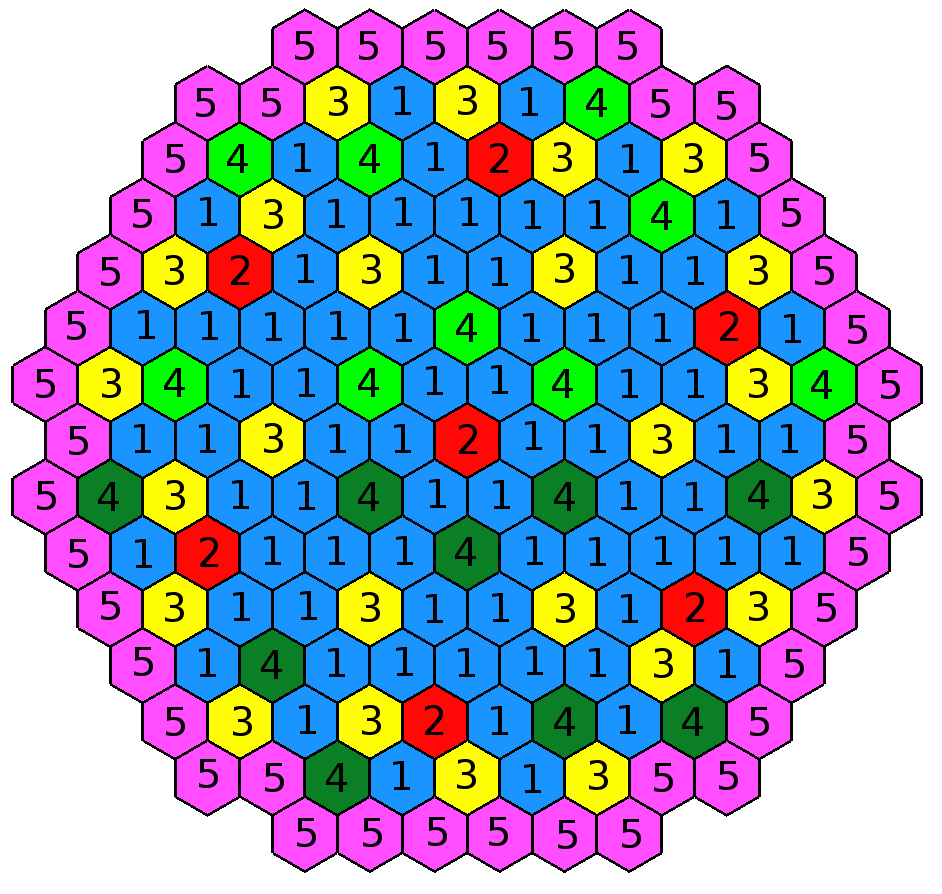
\includegraphics[width=0.75\linewidth] {2.png}
	\caption{Geometrcial model of the VVER-1000 reactor core.}
	\label{fig:2}
  \end{center}
\end{figure} 

Для приближенного решение задачи используется регулярные треугольные сетки.
Число треугольников на одну кассету $\kappa$  варьируется от 6 до 96 (рис.\ref{fig:3}). 

\begin{figure}[!h]
  \begin{center}
\begin{minipage}{0.30\linewidth}
\center{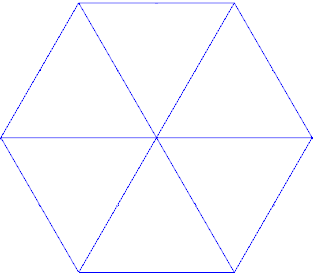
\includegraphics[width=1\linewidth]{3-1.png}}\\
\end{minipage}
\hfill
\begin{minipage}{0.30\linewidth}
\center{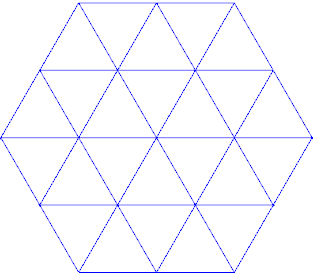
\includegraphics[width=1\linewidth]{3-2.png}}\\
\end{minipage}
\hfill
\begin{minipage}{0.30\linewidth}
\center{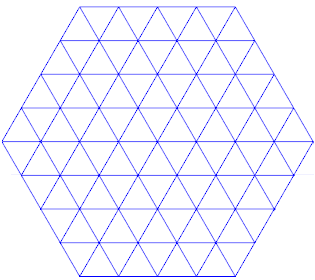
\includegraphics[width=1\linewidth]{3-3.png}}\\
\end{minipage}
\caption{Discretization of assembly into 6, 24 and 96 finite elements.}
\label{fig:3}
  \end{center}
\end{figure}

Используется двухгрупповое приближения с учетом запаздывающих нейтронов, когда 
\begin{equation}\label{22}
\begin{split}
 \frac{1}{v_1}  \frac{\partial \varphi_1}{\partial t}  
 & - \nabla \cdot D_1 \nabla \varphi_1  + \Sigma_1 \varphi_1 + \Sigma_{s,1\rightarrow 2} \varphi_1  \\
 & - (\nu \Sigma_{f1} \varphi_1 + \nu \Sigma_{f2} \varphi_2) - \lambda_1 s = 0, \\
 \frac{1}{v_2}  \frac{\partial \varphi_2}{\partial t}  
 & - \nabla \cdot D_2 \nabla \varphi_2  + \Sigma_2 \varphi_2 - \Sigma_{s,1\rightarrow 2} \varphi_1   = 0,\\
 \frac{\partial s}{\partial t} & + \lambda_1 s - \beta_1(\nu \Sigma_{f1} \varphi_1 + \nu \Sigma_{f2} \varphi_2) = 0. 
\end{split}
\end{equation} 

\begin{table}[htr]
\caption{Diffusion neutronics constants for VVER-1000}
\label{t-1}
\begin{center}
\begin{tabular}{|c|c|c|c|c|c|}
\hline
Материал & 1 & 2 & 3 & 4 & 5\\
\hline
$D_1$ & 1.38320e-0 & 1.38299e-0  & 1.39522e-0  & 1.39446e-0  & 1.39506e-0 \\
$D_2$ & 3.86277e-1 & 3.89403e-1 & 3.86225e-1 & 3.87723e-1 & 3.84492e-1 \\
$\Sigma_1 + \Sigma_{s,1\rightarrow 2}$ & 2.48836e-2 & 2.62865e-2 & 2.45662e-2 & 2.60117e-2 & 2.46141e-2\\
$\Sigma_2$ & 6.73049e-2 & 8.10328e-2 & 8.44801e-1 & 9.89671e-2 & 8.93878e-2\\
$\Sigma_{s,1\rightarrow 2}$ & 1.64977e-2 & 1.47315e-2 & 1.56219e-2 & 1.40185e-2 & 1.54981e-2\\
$\nu\Sigma_{f1}$ & 4.81619e-3 & 4.66953e-3 & 6.04889e-3 & 5.91507e-3 & 6.40256e-3\\
$\nu\Sigma_{f2}$ & 8.46154e-2 & 8.52264e-2 & 1.19428e-1 & 1.20497e-1 & 1.29281e-1\\
\hline
\end{tabular}
\end{center}
\end{table}

Надкритическое состояние реактора характеризуется набором коэффициентов, которые приведены в Table \ref{t-1}. 
Используются граничные условия (\ref{3}) при задании $\gamma_g = 0.5, \ g = 1,2$.  
Характеристики запаздывающих нейтронов: используется одна группа запаздывающих нейтронов 
(эффективная доля $\beta_1 = 6.5\cdot10^{-3}$; постоянная распада $\lambda_1 = 0.08$ с$^{-1}$). 
Скорость нейтронов  $v_1 = 1.25 \cdot 10^7$ см/с и  $v_2 = 2.5 \cdot 10^5$ см/с.

\subsection{Надкритическое состояние: $\alpha$-eigenvalue problem} 

Приведем результаты численного решения $\alpha$-eigenvalue problem (\ref{14}). 
С учетом запаздывающих нейтронов 
в рамках используемого двухгруппового приближения имеем 
\begin{equation}\label{23}
\begin{split}
 - \nabla \cdot D_1 \nabla \varphi_1  + \Sigma_1 \varphi_1 + \Sigma_{s,1\rightarrow 2} \varphi_1  & \\
 - (\nu \Sigma_{f1} \varphi_1 + \nu \Sigma_{f2} \varphi_2) - \lambda_1 s & = \lambda^{(\alpha)} \frac{1}{v_1}   \varphi_1, \\
 - \nabla \cdot D_2 \nabla \varphi_2  + \Sigma_2 \varphi_2  - \Sigma_{s,1\rightarrow 2} \varphi_1  
 & = \lambda^{(\alpha)} \frac{1}{v_2}   \varphi_2,\\
 \lambda_1 s - \beta_1(\nu \Sigma_{f1} \varphi_1 + \nu \Sigma_{f2} \varphi_2) & = \lambda^{(\alpha)} s. 
\end{split}
\end{equation} 
Ищутся dominant собственное значение $\alpha_n = \lambda_n^{(\alpha)}, \ n = 1,2, ..., N$ при
\[
 \mathrm{Re}  \lambda_1^{(\alpha)} \leq  \mathrm{Re}  \lambda_2^{(\alpha)} \leq ... 
 \leq \mathrm{Re}  \lambda_N^{(\alpha)} \leq ...\, \leq \mathrm{Re}  \lambda_{N_h}^{(\alpha)}.
\]
Аналогичные расчеты собственных значений реактора VVER-1000 без учета запаздывающих
нейтронов можно найти в работе \cite{avvakumov2017spectral}. 

\begin{table}[h]
\caption{Собственные значения $\alpha_n = \lambda_n^{(\alpha )}, \ n = 1,2, ..., 5$}
\label{t-2}
\begin{center}
\begin{tabular}{cccccc}
\hline
$p$ & $\kappa$ & $\alpha_1$ &  $\alpha_2, \alpha_3$ &  $\alpha_4, \alpha_5$ \\ 
\hline
& 6 & -0.22557  & 0.04241 $\mp$ 3.08808e-06$i$  & 0.06588 $\mp$ 4.80449e-07$i$  \\
1 & 24 & -0.82690  & 0.03777 $\mp$ 5.37884e-06$i$  & 0.06489 $\mp$ 1.37315e-06$i$ \\
& 96 & -1.74998  & 0.03619 $\mp$ 5.69002e-06$i$  & 0.06456 $\mp$ 1.40299e-06$i$ \\
\hline
& 6 & -2.10154  & 0.03592 $\mp$ 4.96474e-06$i$  & 0.06452 $\mp$ 1.21320e-06$i$ \\
2 & 24 & -2.46601  & 0.03562 $\mp$ 5.78277e-06$i$  & 0.06445 $\mp$ 1.40897e-06$i$ \\
& 96 & -2.50375  & 0.03559 $\mp$ 5.80693e-06$i$  & 0.06444 $\mp$ 1.41324e-06$i$ \\
\hline
& 6 & -2.47975  & 0.03561 $\mp$ 5.83718e-06$i$  & 0.06445 $\mp$ 1.41869e-06$i$ \\
3 & 24 & -2.50294  & 0.03559 $\mp$ 5.80783e-06$i$  & 0.06444 $\mp$ 1.41341e-06$i$ \\
& 96 & -2.51280  & 0.03558 $\mp$ 5.80954e-06$i$  & 0.06444 $\mp$ 1.41362e-06$i$ \\
\hline
\end{tabular}
\end{center}
\end{table}

\begin{table}[h]
\caption{Собственные значения $\alpha_n = \lambda_n^{(\alpha )}, \ n = 6,7, ..., 10$}
\label{t-3}
\begin{center}
\begin{tabular}{ccccccc}
\hline
$p$ & $\kappa$ & $\alpha_6$ &  $\alpha_7$ & $\alpha_8$ &  $\alpha_9, \alpha_{10}$ \\ 
\hline
& 6 & 0.07107  & 0.07214  & 0.07323  & 0.07397 $\mp$ 2.04990e-08$i$ \\
1 & 24 & 0.07050  & 0.07167  & 0.07283  & 0.07362 $\mp$ 3.65907e-08$i$ \\
& 96 & 0.07033  & 0.07152  & 0.07269  & 0.07351 $\mp$ 3.91936e-08$i$  \\
\hline
& 6  & 0.07030  & 0.07151  & 0.07268  & 0.07349 $\mp$ 3.69824e-08$i$ \\
2 & 24 & 0.07027  & 0.07147  & 0.07265  & 0.07347 $\mp$ 4.03121e-08$i$ \\
& 96  & 0.07026  & 0.07147  & 0.07265  & 0.07347 $\mp$ 4.02324e-08$i$ \\
\hline
& 6 & 0.07027  & 0.07147  & 0.07265  & 0.07347 $\mp$ 4.02573e-08$i$ \\
3 & 24 & 0.07026  & 0.07147  & 0.07265  & 0.07347 $\mp$ 4.02248e-08$i$ \\
& 96 & 0.07026  & 0.07147  & 0.07265  & 0.07347 $\mp$ 4.02332e-08$i$ \\
\hline
\end{tabular}
\end{center}
\end{table}

Результаты решения спектральной задачи (\ref{23}) для первых собственных
значений $\alpha_n = \lambda_n^{(\alpha)}, \ n = 1,2, ..., N$, $ N=10$
на разных расчетных сетках при использовании различных
конечно-элементных аппроксимаций показаны в табл.\ref{t-2}, \ref{t-3}. Cобственные значения $\alpha_2, \alpha_3$, $\alpha_4, \alpha_5$, $\alpha_9, \alpha_{10}$ 
для спектральной задачи (\ref{23}) являются комплексные с малыми мнимыми частями, собственные значения $\alpha_1, \alpha_6$, $\alpha_7, \alpha_8$ --- действительные.

В нашем примере главное собственное значение
отрицательно и поэтому главная гармоника
будет нарастать, а все другие будут затухать. Тем самым выражен регулярный режим 
работы реактора. Сама величина $\alpha = \lambda_1^{(\alpha)}$ определяет амплитуду 
развития нейтронного поля и непосредственно связывается с периодом реактора
в регулярном режиме.

\begin{figure}[!h]
  \begin{center}
\begin{minipage}{0.49\linewidth}
\center{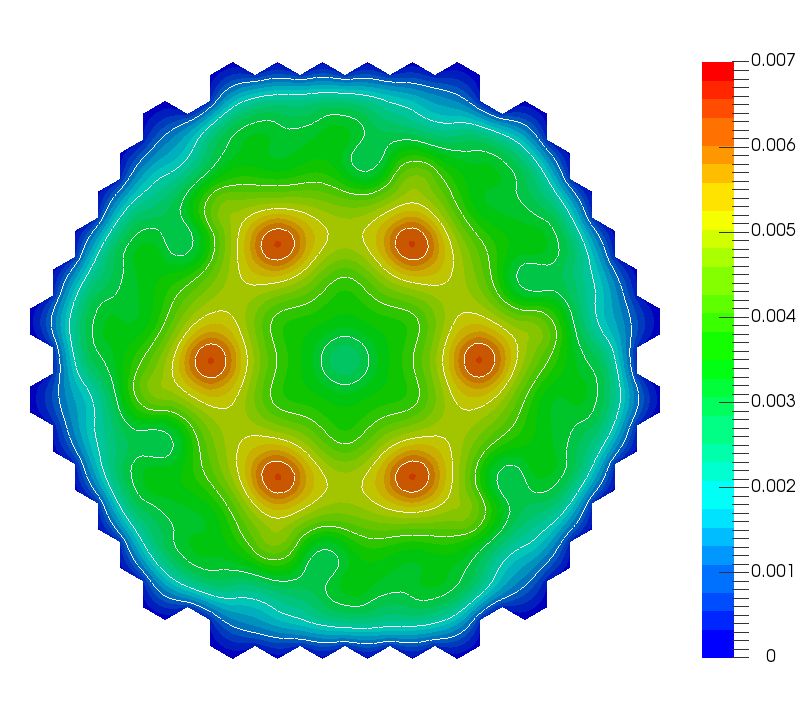
\includegraphics[width=1\linewidth]{4-1.png}} \\
\end{minipage}
\hfill
\begin{minipage}{0.49\linewidth}
\center{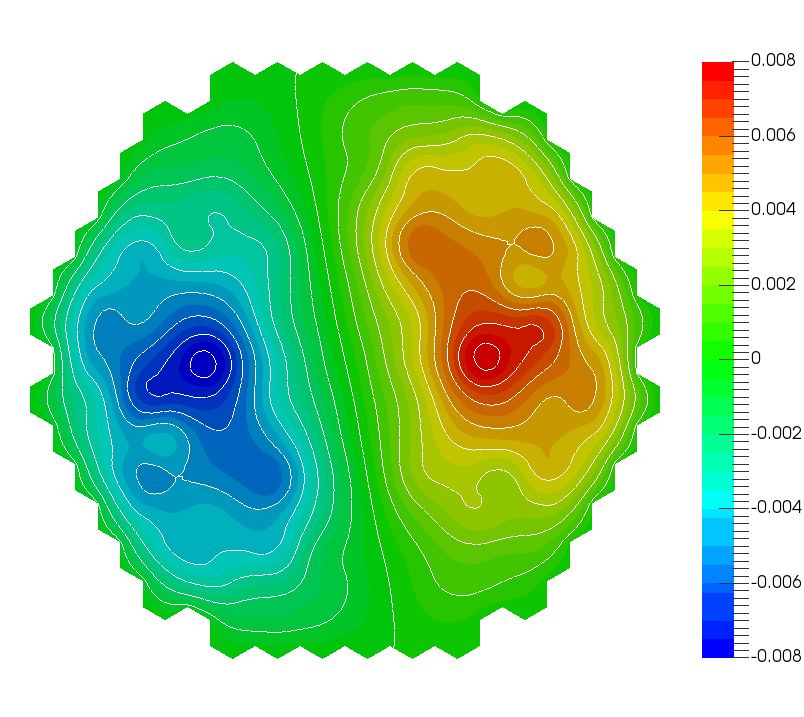
\includegraphics[width=1\linewidth]{4-2.png}} \\
\end{minipage}
\caption{The eigenfunction $\varphi^{(1)}_1$ (left) and real part of eigenfunctions $\varphi^{(2)}_1, \ \varphi^{(3)}_1$  (right).}
\label{fig:4}
  \end{center}
\end{figure}

\begin{figure}[!h]
  \begin{center}
\begin{minipage}{0.49\linewidth}
\center{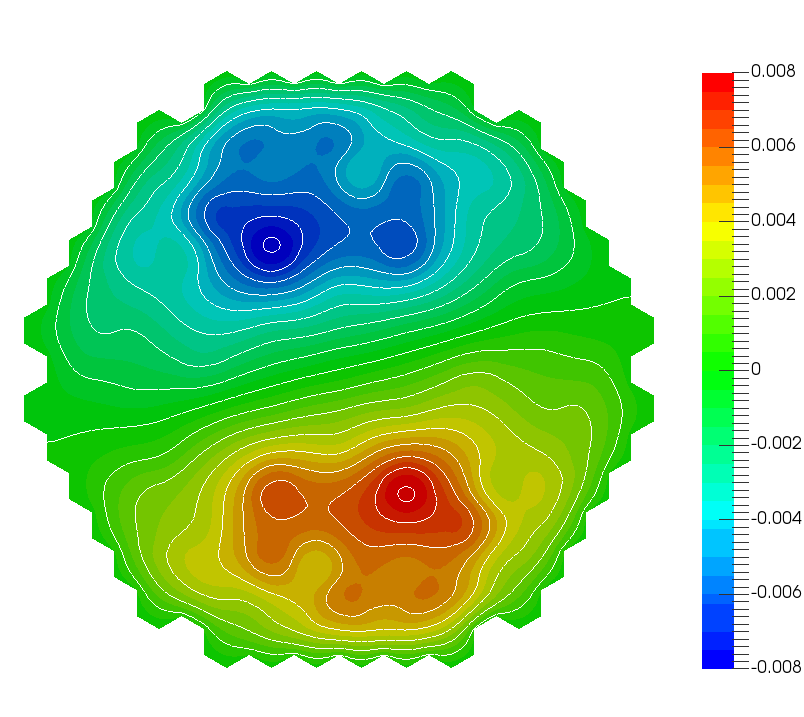
\includegraphics[width=1\linewidth]{5-1.png}} \\
\end{minipage}
\hfill
\begin{minipage}{0.49\linewidth}
\center{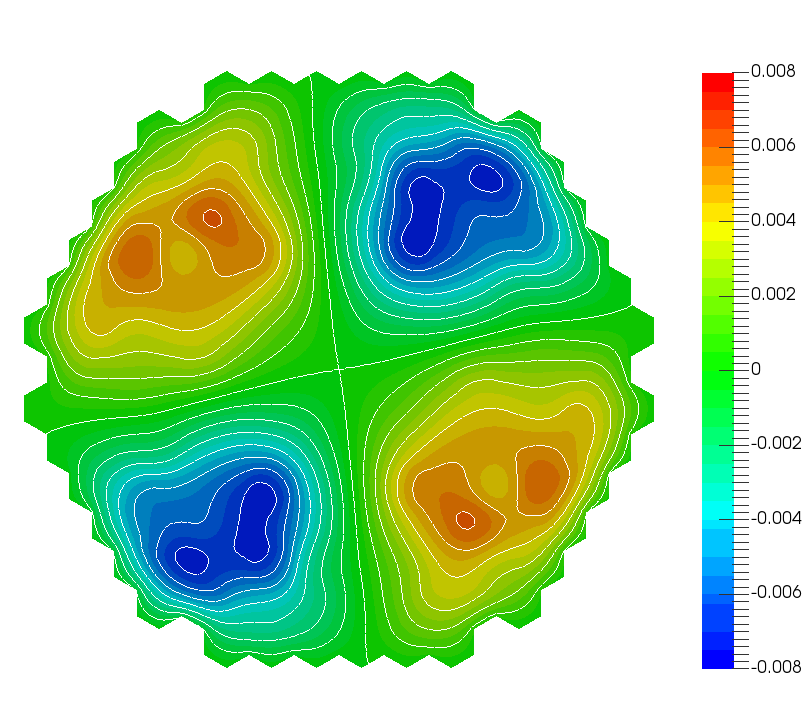
\includegraphics[width=1\linewidth]{5-2.png}} \\
\end{minipage}
\caption{Imaginary part of eigenfunctions $\varphi^{(2)}_1, \ - \varphi^{(3)}_1$ (left) and  real part of eigenfunctions $\varphi^{(4)}_1, \ \varphi^{(5)}_1$  (right).}
\label{fig:5}
  \end{center}
\end{figure}

\begin{figure}[!h]
  \begin{center}
\begin{minipage}{0.49\linewidth}
\center{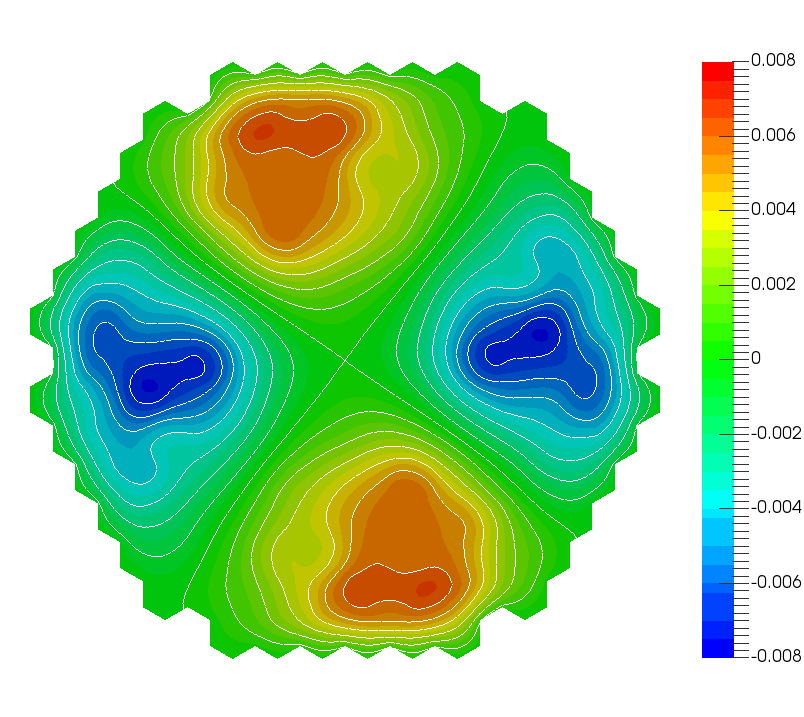
\includegraphics[width=1\linewidth]{6-1.png}} \\
\end{minipage}
\hfill
\begin{minipage}{0.49\linewidth}
\center{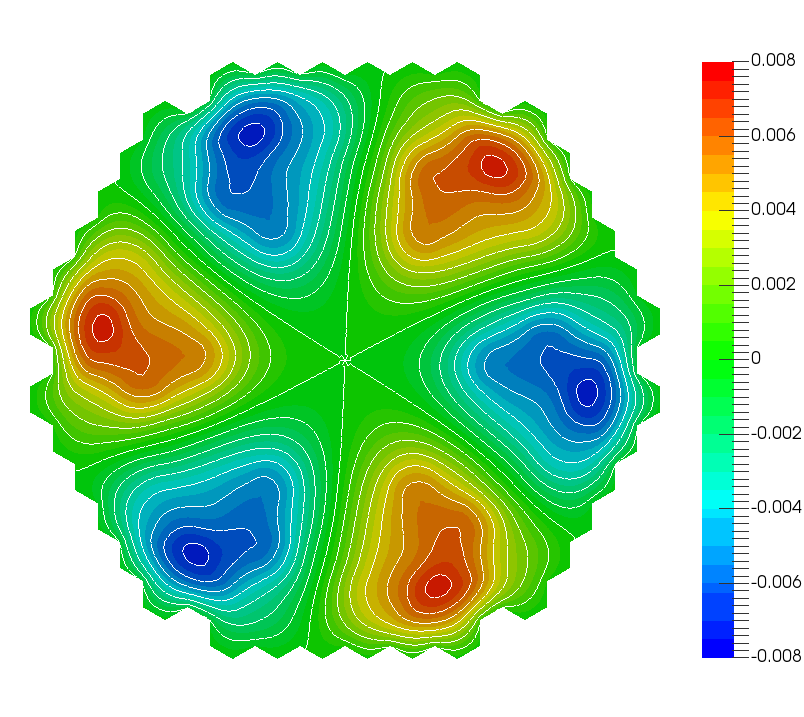
\includegraphics[width=1\linewidth]{6-2.png}} \\
\end{minipage}
\caption{Imaginary part of eigenfunctions $\varphi^{(4)}_1, \ - \varphi^{(5)}_1$ (left) and  eigenfunction $\varphi^{(6)}_1$  (right).}
\label{fig:6}
  \end{center}
\end{figure}

\begin{figure}[!h]
  \begin{center}
\begin{minipage}{0.49\linewidth}
\center{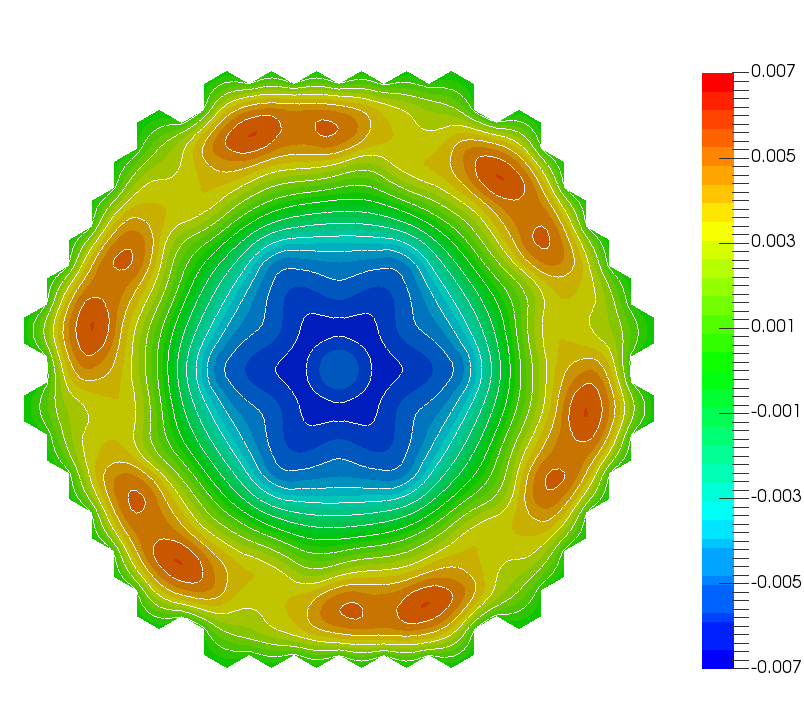
\includegraphics[width=1\linewidth]{7-1.png}} \\
\end{minipage}
\hfill
\begin{minipage}{0.49\linewidth}
\center{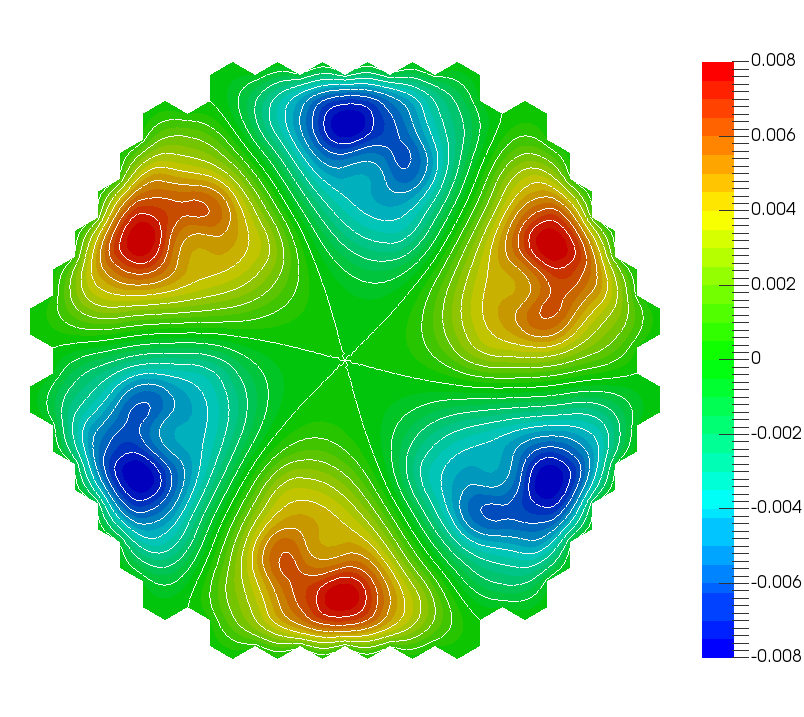
\includegraphics[width=1\linewidth]{7-2.png}} \\
\end{minipage}
\caption{The eigenfunction $\varphi^{(7)}_1$ (left) and  eigenfunction $\varphi^{(8)}_1$  (right).}
\label{fig:7}
  \end{center}
\end{figure}

\begin{figure}[!h]
  \begin{center}
\begin{minipage}{0.49\linewidth}
\center{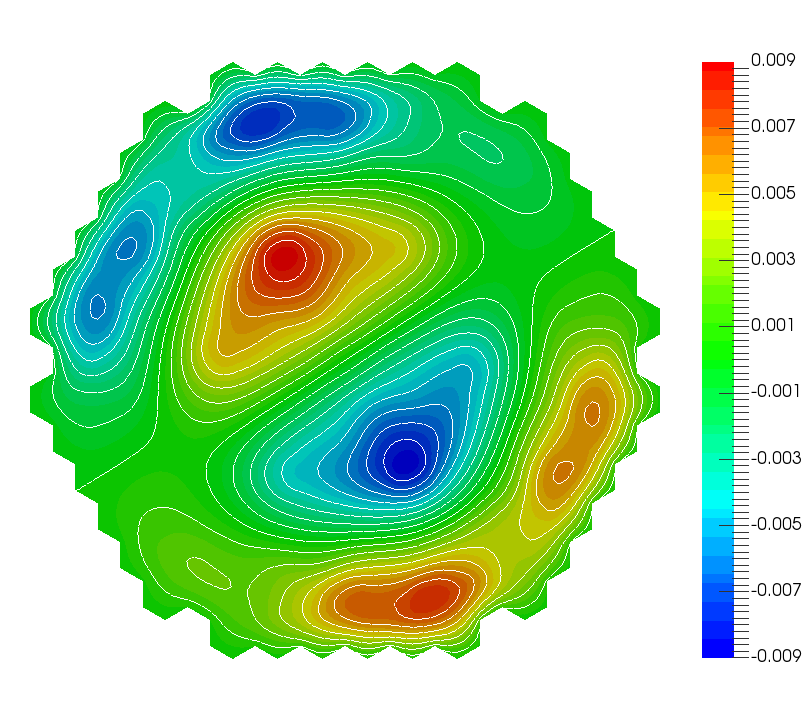
\includegraphics[width=1\linewidth]{8-1.png}} \\
\end{minipage}
\hfill
\begin{minipage}{0.49\linewidth}
\center{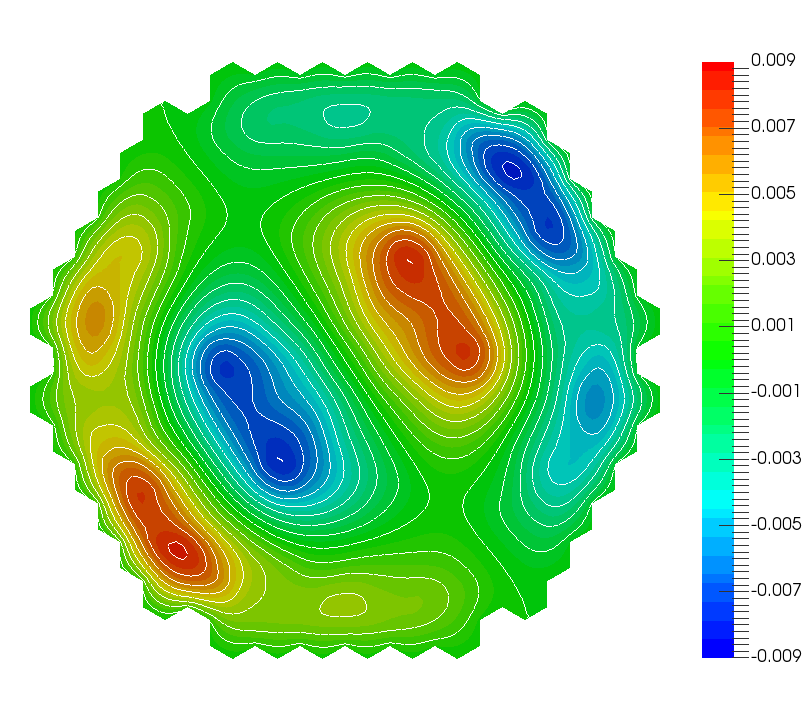
\includegraphics[width=1\linewidth]{8-2.png}} \\
\end{minipage}
\caption{Real part of eigenfunctions $\varphi^{(9)}_1, \ \varphi^{(10)}_1$ (left) and  imaginary part of eigenfunctions $\varphi^{(9)}_1, \ - \varphi^{(10)}_1$  (right).}
\label{fig:8}
  \end{center}
\end{figure}

Dominant собственные функции спектральной задачи (\ref{23}) для группы 1 показаны рис.\ref{fig:4}--\ref{fig:8}. 
Расчеты выполнены на сетке с $\kappa=96$ с использованием конечных элементов степени $p=3$.
Главные собственные функции для второй группы $\varphi^{(1)}_2$ и запаздывающих нейтронов $s^{(1)}$  показаны на  
рис.\ref{fig:9}. 

\begin{figure}[!h]
  \begin{center}
\begin{minipage}{0.49\linewidth}
\center{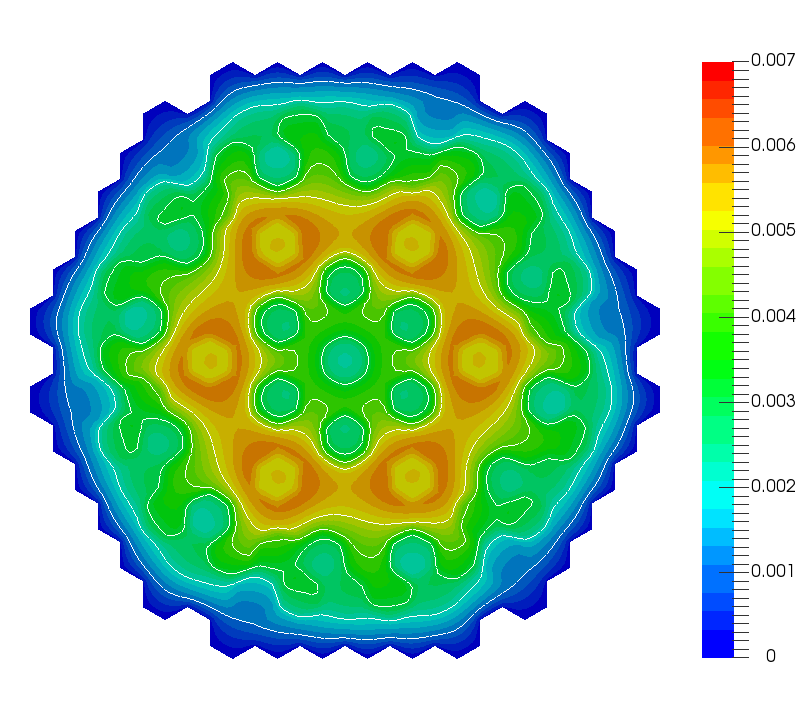
\includegraphics[width=1\linewidth]{9-1.png}} \\
\end{minipage}
\hfill
\begin{minipage}{0.49\linewidth}
\center{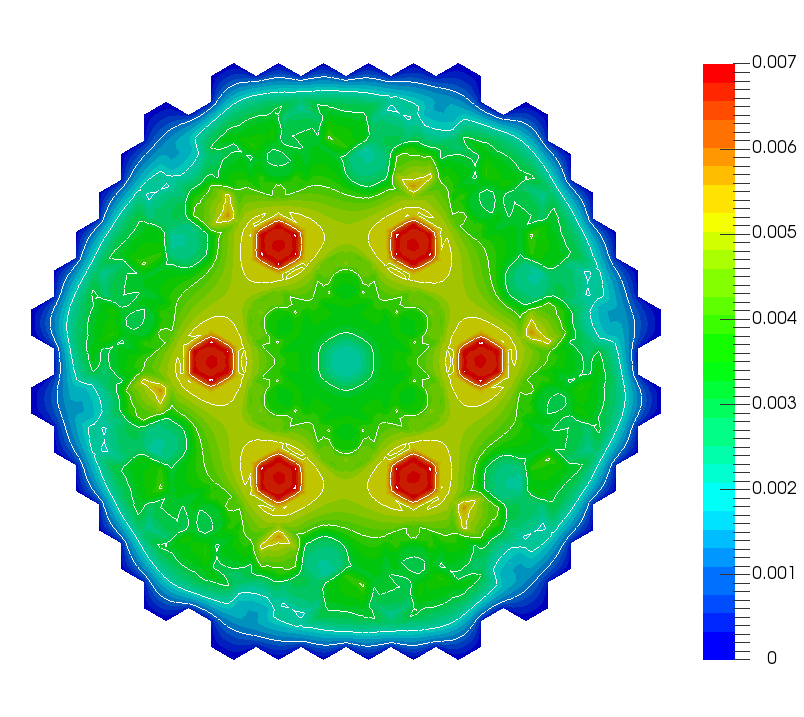
\includegraphics[width=1\linewidth]{9-2.png}} \\
\end{minipage}
\caption{The eigenfunction $\varphi^{(1)}_2$ (left) and the eigenfunctions $s^{(1)}$  (right).}
\label{fig:9}
  \end{center}
\end{figure}

\begin{table}[h]
\caption{Собственные значения $\alpha_n = \lambda_n^{(\alpha )}, \ n = 1,2, ..., 10$
основной и сопряженной задач}
\label{t-4}
\begin{center}
\begin{tabular}{rll}
\hline
$n$ & $\alpha_n$ для задачи (\ref{14}) & $\alpha_n$ для задачи (\ref{16}) \\
\hline
1 & -2.51280117966 & -2.51280117972 \\
2,3 & 0.0355815000364 $\mp$ 5.80954455861e-06 & 0.0355815000365 $\mp$ 5.80954421646e-06 \\
4,5 & 0.0644427013767 $\mp$ 1.41362187449e-06 & 0.0644427013767 $\mp$ 1.41362190730e-06 \\
6 & 0.0702618501639 & 0.0702618501639 \\
7 & 0.0714652882224 & 0.0714652882164 \\
8 & 0.0726456060606 & 0.0726456060606 \\
9,10 & 0.0734708921578 $\mp$ 4.02332269037e-08 & 0.0734708921578 $\mp$ 4.02332146248e-08 \\
\hline
\end{tabular}
\end{center}
\end{table}

\subsection{Сопряженная спектральная задача} 

Аналогичные данные получены при приближенном решении сопряженной спектральной задачи (\ref{16}).
Собственные значения спектральных задач (\ref{14}) и (\ref{16}) совпадают.
Их отличие друг от друга является косвенной мерой точности численного решения.
Данные по dominant собственным значениям, которые приведены в Table \ref{t-4} ($k=96, \ p = 3$), показывают, что
собственные значения основной и сопряженной спектральных задач близки друг к другу
с хорошей точностью. 

Рассматриваемые спектральные задачи характеризуются
небольшими значениями мнимых частей собственных значений. 
В силу этого мы можем рассчитывать на то, что собственные функции задачи (\ref{14}) 
близки к ортогональным. Иллюстрацией служит Table \ref{t-5}, в которой 
приведены данные для скалярных произведений $(\phi_1^{(n)}, \phi_1^{(m)})$
для первых 10 собственных функций. Для удобства сравнения
собственные функции нормированы в $L_2(\Omega)$:
\[
 \phi_1^{(n)} \longrightarrow \frac{\phi_1^{(n)}}{\|\phi_1^{(n)}\|} .
\] 
Наибольшая неортогональность (для $(\phi_1^{(1)}, \phi_1^{(7)})$)
не превышает 10 \%.
Примерно с этой же точностью выполняется и условие биортогональности собственных
функций основной (смотри (\ref{14})) и сопряженной (смотри (\ref{16}))
спектральных задач.
Эту наблюдаемую погрешность можно связать с приближенным вычислением собственных значений и собственным функций.

\begin{table}[h]
\caption{Скалярное произведение $(\phi_1^{(n)}, \phi_1^{(m)}), \ n, m = 1,2, ..., 10$}
\label{t-5}
\begin{center}
\footnotesize 
%\small
\begin{tabular}{c|rrrrrrrrrr}
\hline
$n$\textbackslash$m$&1&2&3&4&5&6&7&8&9&10 \\
\hline
1 & 1.0e-00 & 1.3e-08 & 2.2e-08 & -3.8e-08 & 9.8e-09 & -1.8e-09 & 1.0e-02 & -3.2e-09 & -2.2e-08 & 1.6e-09 \\ 
2 & 1.3e-08 & 1.0e-00 & -1.6e-08 & -1.6e-08 & 1.4e-08 & 4.1e-08 & 1.2e-09 & -2.0e-07 & -3.1e-03 & 7.5e-03 \\ 
3 & 2.2e-08 & -1.6e-08 & 1.0e-00 & -9.8e-09 & -1.1e-08 & -1.8e-08 & 1.1e-08 & -3.3e-08 & -7.5e-03 & -3.1e-03 \\ 
4 & -3.8e-08 & -1.6e-08 & -9.8e-09 & 1.0e-00 & -3.9e-10 & -1.1e-08 & 1.4e-08 & 4.0e-09 & 3.0e-09 & -1.1e-08 \\ 
5 & 9.8e-09 & 1.4e-08 & -1.1e-08 & -3.9e-10 & 1.0e-00 & 2.9e-09 & -1.6e-08 & -1.9e-08 & 6.3e-09 & 6.3e-09 \\ 
6 & -1.8e-09 & 4.1e-08 & -1.8e-08 & -1.1e-08 & 2.9e-09 & 1.0e-00 & -4.2e-09 & -5.6e-03 & 4.1e-08 & -1.2e-07 \\ 
7 & 1.0e-02 & 1.2e-09 & 1.1e-08 & 1.4e-08 & -1.6e-08 & -4.2e-09 & 1.0e-00 & -2.1e-09 & -1.8e-08 & 8.0e-09 \\ 
8 & -3.2e-09 & -2.0e-07 & -3.3e-08 & 4.0e-09 & -1.9e-08 & -5.6e-03 & -2.1e-09 & 1.0e-00 & -5.2e-08 & 2.3e-07 \\ 
9 & -2.2e-08 & -3.1e-03 & -7.5e-03 & 3.0e-09 & 6.3e-09 & 4.1e-08 & -1.8e-08 & -5.2e-08 & 1.0e-00 & -5.5e-07 \\ 
10 & 1.6e-09 & 7.5e-03 & -3.1e-03 & -1.1e-08 & 6.3e-09 & -1.2e-07 & 8.0e-09 & 2.3e-07 & -5.5e-07 & 1.0e-00 \\ 
\hline
\end{tabular}
\end{center}
\end{table}

В рамках modal method мы не можем рассчитывать на высокую точность при 
учете относительно небольшого числа dominant собственных значений.
В силу этого в рассматриваемом примере мы можем считать, что собственные значения действительны,
а соответствующие им собственные функции --- ортогональными. 
Вместо (\ref{17}) используются коэффициенты
\begin{equation}\label{24}
 b_n \approx  \frac{1}{(\bm c_n, \bm c_n)} (\bm c_h^s, \bm c_n),
 \quad n = 1,2, ..., N ,
\end{equation}
для аппроксимации начального условия.

\subsection{Подкритическое состояние} 

В надкритическом режиме в силу достаточно большой величины по модулю главного собственного значения
быстро развивается регулярный режим реактора, в котором 
\[
 \bm u (\bm x, t) \approx a_1 \exp(-\alpha_1 t) \bm v_1^0 (\bm x) .
\] 
Здесь $\bm v_1^0 (\bm x)$ есть первая мода надкритического состояния.
Рассмотрим задачу с переходом из этого надкритического состояния при $t_0 = 0$  в подкритический.

Подкритическая стадия характеризуется увеличением на  15\% коэффициента 
$\Sigma_2$ в diffusion neutronics constants for VVER-1000  для материала 4 (see Table \ref{t-1}). 
Тем самым рассматривается динамика реактора при 
\[
 \Sigma_2 \longrightarrow 1.15 \Sigma_2 \quad (\mathrm{material} \ 4).
\] 
Начальное состояние характеризуется заданием начальных условий (\ref{8}) 
при $t_0 = 0$ в виде
\begin{equation}\label{25}
 \bm u (\bm x, 0) = \bm v_1^0 (\bm x) . 
\end{equation} 

Результаты расчетов dominant собственных значений поктритического состояния реактора
представлены в Tables \ref{t-6}, \ref{t-7}. В этом случае даже первые 
собственные значения менее сильно отличаются друг от друга. 

\begin{table}[h]
\caption{Подкритическое состояние: $\alpha_n = \lambda_n^{(\alpha )}, \ n = 1,2, ..., 5$}
\label{t-6}
\begin{center}
\begin{tabular}{cccccc}
\hline
$p$ & $\kappa$ & $\alpha_1$ &  $\alpha_2, \alpha_3$ &  $\alpha_4, \alpha_5$ \\ 
\hline
   & 6 & 0.03602 & 0.05760 $\mp$ 1.49652e-06$i$ & 0.06890 $\mp$ 4.92606e-07$i$ \\ 
1 & 24 & 0.02656 & 0.05502 $\mp$ 2.06007e-06$i$ & 0.06804 $\mp$ 1.01253e-06$i$ \\ 
  & 96 & 0.02276 & 0.05411 $\mp$ 2.16813e-06$i$ & 0.06774 $\mp$ 1.03843e-06$i$ \\ 
\hline
   & 6 & 0.02250 & 0.05404 $\mp$ 1.81823e-06$i$ & 0.06772 $\mp$ 8.73562e-07$i$ \\ 
2 & 24 & 0.02144 & 0.05380 $\mp$ 2.19400e-06$i$ & 0.06765 $\mp$ 1.04253e-06$i$ \\ 
  & 96 & 0.02125 & 0.05376 $\mp$ 2.20812e-06$i$ & 0.06763 $\mp$ 1.04715e-06$i$ \\ 
\hline
   & 6 & 0.02139 & 0.05379 $\mp$ 2.22579e-06$i$ & 0.06764 $\mp$ 1.05369e-06$i$ \\ 
3 & 24 & 0.02124 & 0.05376 $\mp$ 2.20883e-06$i$ & 0.06763 $\mp$ 1.04736e-06$i$ \\ 
  & 96 & 0.02122 & 0.05376 $\mp$ 2.20951e-06$i$ & 0.06763 $\mp$ 1.04756e-06$i$ \\ 
\hline
\end{tabular}
\end{center}
\end{table}

\begin{table}[h]
\caption{Подкритическое состояние:  $\alpha_n = \lambda_n^{(\alpha )}, \ n = 6,7, ..., 10$}
\label{t-7}
\begin{center}
\begin{tabular}{ccccccc}
\hline
$p$ & $\kappa$ & $\alpha_6$ &  $\alpha_7$ & $\alpha_8$ &  $\alpha_9, \alpha_{10}$ \\ 
\hline
   & 6 & 0.07276 & 0.07363 & 0.07369 & 0.07466 $\mp$ 2.47162e-08$i$ \\ 
1 & 24 & 0.07222 & 0.07316 & 0.07329 & 0.07429 $\mp$ 1.08814e-08$i$ \\ 
  & 96 & 0.07204 & 0.07301 & 0.07316 & 0.07417 $\mp$ 1.38093e-08$i$ \\
\hline
   & 6 & 0.07203 & 0.07300 & 0.07315 & 0.07416 $\mp$ 1.26708e-08$i$ \\ 
2 & 24 & 0.07199 & 0.07296 & 0.07312 & 0.07413 $\mp$ 1.50527e-08$i$ \\ 
  & 96 & 0.07198 & 0.07295 & 0.07312 & 0.07413 $\mp$ 1.49196e-08$i$ \\ 
\hline
   & 6 & 0.07198 & 0.07295 & 0.07312 & 0.07413 $\mp$ 1.52256e-08$i$ \\ 
3 & 24 & 0.07198 & 0.07295 & 0.07312 & 0.07413 $\mp$ 1.49141e-08$i$ \\ 
  & 96 & 0.07198 & 0.07295 & 0.07311 & 0.07413 $\mp$ 1.49178e-08$i$ \\ 
\hline
\end{tabular}
\end{center}
\end{table}

Для приближенного решения используется представление
\begin{equation}\label{26}
 \bm u_N(\bm x, t) = 
 \sum_{n=1}^{N} b_n \exp(- \mathrm{Re} \, \alpha_n \, t) \bm v_n(\bm x) ,  
\end{equation} 
в котором коэффициенты $b_n, \ n = 1,2, ..., N$ рассчитываются по заданному начальному
условию согласно (\ref{24}). Эти коэффициенты для $N=50$ показаны на рис.\ref{fig:10}. 
Как мы видим, приближенное решение может быть описано только одной первой модой.

\begin{figure}[!h]
  \begin{center}
    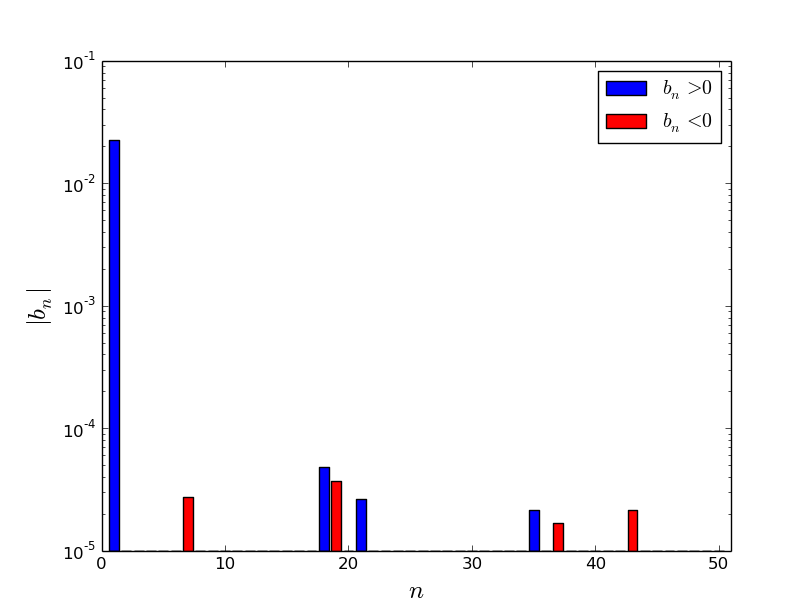
\includegraphics[width=0.95\linewidth] {10.png}
	\caption{Коэффициенты для приближенного решения (\ref{26}).}
	\label{fig:10}
  \end{center}
\end{figure} 

Мы выделяем две фазы динамического процесса: быстрая и медленная.
На быстрой фазе происходит перестройка начального условия (\ref{25}) 
к начальному условию, которое соответствует (\ref{26}): от функции
$\bm u(\bm x, 0)$ к функции $\bm u_N(\bm x, 0)$. Медленная фаза связывается с эволюцией
решения согласно (\ref{26}).
В рамках state change modal технологии выделенная быстрая фаза не моделируется.

Начало и конец быстрой фазы иллюстрируется расчетными данными на рис.\ref{fig:11},
которые получены при $N=10$. Мы можем отметить непринципиальные изменения 
топологии исходных и перестроенных начальных условий. 
Обратим внимание на существенную перестройку решения, которая
иллюстрируется большими изменениями амплитуд нейтронов первой и второй групп.

\begin{figure}[!h]
  \begin{center}
\begin{minipage}{0.051\linewidth}
\center{1} \\
\end{minipage}
\hfill
\begin{minipage}{0.3\linewidth}
\center{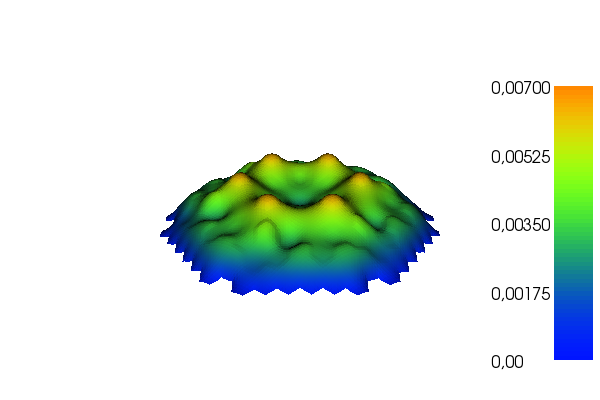
\includegraphics[width=1\linewidth]{11-11.png}} \\
\end{minipage}
\hfill
\begin{minipage}{0.3\linewidth}
\center{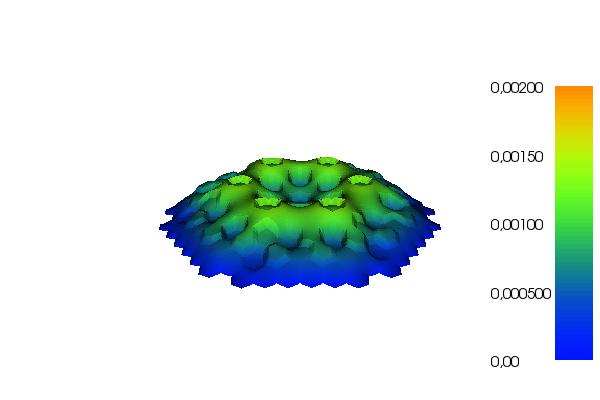
\includegraphics[width=1\linewidth]{11-12.png}} \\
\end{minipage}
\hfill
\begin{minipage}{0.3\linewidth}
\center{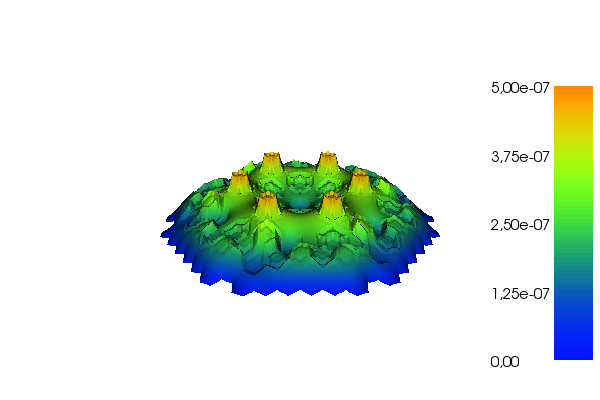
\includegraphics[width=1\linewidth]{11-13.png}} \\
\end{minipage}

\begin{minipage}{0.051\linewidth}
\center{2} \\
\end{minipage}
\hfill
\begin{minipage}{0.3\linewidth}
\center{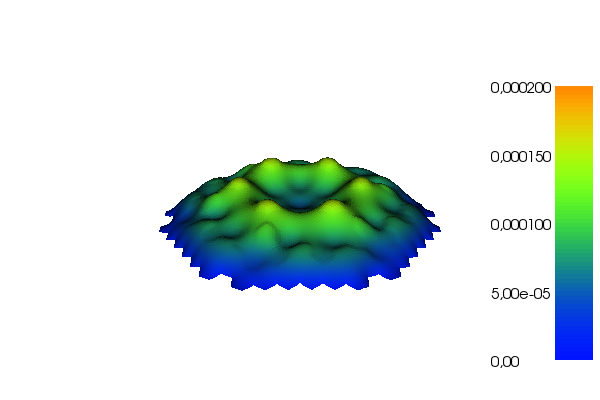
\includegraphics[width=1\linewidth]{11-21.png}} \\
\end{minipage}
\hfill
\begin{minipage}{0.3\linewidth}
\center{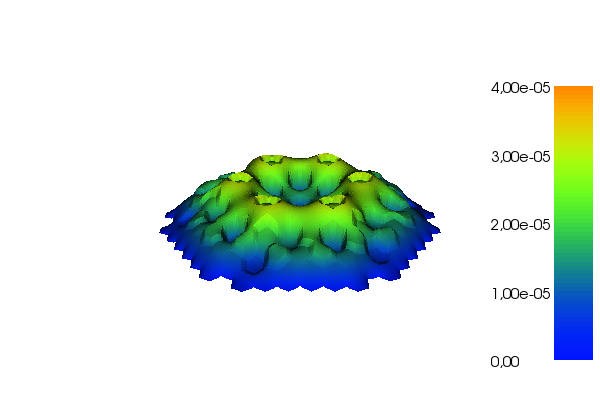
\includegraphics[width=1\linewidth]{11-22.png}} \\
\end{minipage}
\hfill
\begin{minipage}{0.3\linewidth}
\center{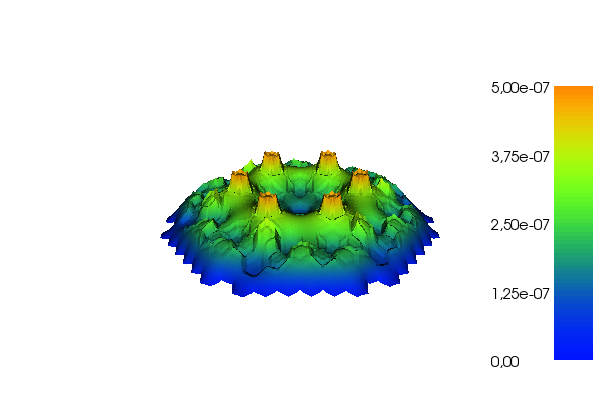
\includegraphics[width=1\linewidth]{11-23.png}} \\
\end{minipage}

\begin{minipage}{0.051\linewidth}
\center{ } \\
\end{minipage}
\hfill
\begin{minipage}{0.3\linewidth}
\center{a} \\
\end{minipage}
\hfill
\begin{minipage}{0.3\linewidth}
\center{b} \\
\end{minipage}
\hfill
\begin{minipage}{0.3\linewidth}
\center{c} \\
\end{minipage}
\hfill

\caption{Функция $\bm u(\bm x, 0)$ (строка 1) и функция  $\bm u_N(\bm x, 0)$ (строка 2):
a --- neutron flux of 1 group, b --- neutron flux of 2 group, c --- delayed neutron.}
\label{fig:11}
  \end{center}
\end{figure}

\subsection{Несимметричное возмущение} 

Рассмотрим более сложный переход в подкритическое состояние.
Подкритическую стадию будем характеризовать 
разным увеличением коэффициента 
$\Sigma_2$ в diffusion neutronics constants  для материала 4 в верхней и нижней половине сечения реактора
(see рис.\ref{fig:2}). Пусть теперь динамика реактора соответствует трансформации
\[
 \Sigma_2 \longrightarrow 
 \begin{cases}
 1.1 \Sigma_2, & \mathrm{material \ 4 \ (top \ part)}, \\
 1.2 \Sigma_2, & \mathrm{material \ 4 \ (bottom \ part)}.
 \end{cases}
\] 

Результаты расчетов dominant собственных значений подкритического состояния реактора
при несимметричном возмущении представлены в Tables \ref{t-8}, \ref{t-9}. Все
собственные значения для этого состояния реактора являются действительными. 

\begin{table}[h]
\caption{Подкритическое несимметричное состояние: $\alpha_n = \lambda_n^{(\alpha )}, \ n = 1,2, ..., 5$}
\label{t-8}
\begin{center}
\begin{tabular}{ccccccc}
\hline
$p$ & $\kappa$ & $\alpha_1$ &  $\alpha_2$ & $\alpha_3$ &  $\alpha_4$ & $\alpha_5$ \\ 
\hline
   & 6 & 0.03347 & 0.05728 & 0.05788 & 0.06884 & 0.06889 \\ 
1 & 24 & 0.02333 & 0.05467 & 0.05528 & 0.06797 & 0.06802 \\ 
  & 96 & 0.01925 & 0.05374 & 0.05436 & 0.06768 & 0.06772 \\ 
\hline
   & 6 & 0.01894 & 0.05367 & 0.05429 & 0.06765 & 0.06770 \\ 
2 & 24 & 0.01782 & 0.05343 & 0.05405 & 0.06758 & 0.06762 \\ 
  & 96 & 0.01763 & 0.05339 & 0.05401 & 0.06757 & 0.06761 \\ 
\hline
   & 6 & 0.01777 & 0.05342 & 0.05404 & 0.06758 & 0.06762 \\ 
3 & 24 & 0.01762 & 0.05339 & 0.05400 & 0.06757 & 0.06761 \\ 
  & 96 & 0.01760 & 0.05338 & 0.05400 & 0.06757 & 0.06761 \\ 
\hline
\end{tabular}
\end{center}
\end{table}

\begin{table}[h]
\caption{Подкритическое несимметричное состояние:  $\alpha_n = \lambda_n^{(\alpha )}, \ n = 6,7, ..., 10$}
\label{t-9}
\begin{center}
\begin{tabular}{cccccccc}
\hline
$p$ & $\kappa$ & $\alpha_6$ &  $\alpha_7$ & $\alpha_8$ &  $\alpha_9$ & $\alpha_{10}$ \\  
\hline
   & 6 & 0.07274 & 0.07355 & 0.07369 & 0.07464 & 0.07468 \\ 
1 & 24 & 0.07220 & 0.07309 & 0.07329 & 0.07427 & 0.07430 \\
  & 96 & 0.07202 & 0.07294 & 0.07316 & 0.07415 & 0.07419 \\ 
\hline
   & 6 & 0.07201 & 0.07293 & 0.07314 & 0.07414 & 0.07417 \\
2 & 24 & 0.07197 & 0.07289 & 0.07311 & 0.07412 & 0.07415 \\ 
  & 96 & 0.07196 & 0.07288 & 0.07311 & 0.07411 & 0.07414 \\ 
\hline
   & 6 & 0.07196 & 0.07289 & 0.07311 & 0.07411 & 0.07415 \\ 
3 & 24 & 0.07196 & 0.07288 & 0.07311 & 0.07411 & 0.07414 \\ 
  & 96 & 0.07196 & 0.07288 & 0.07311 & 0.07411 & 0.07414 \\ 
\hline
\end{tabular}
\end{center}
\end{table}

Коэффициенты $b_n, \ n = 1,2, ..., N$, $N=50$ для приближенного
решения (\ref{26}) при начальном условии (\ref{25}) приведены на рис.\ref{fig:12}. 
В рассматриваемом случае приближенное решение содержит группу мод и не может быть
описано только первой модой. Быстрая фаза перехода иллюстрируется рис.\ref{fig:11},
Расчеты конца быстрой фазы (функции $\bm u_N(\bm x, 0)$) выполнены при 
$N=10$. 

\begin{figure}[!h]
  \begin{center}
    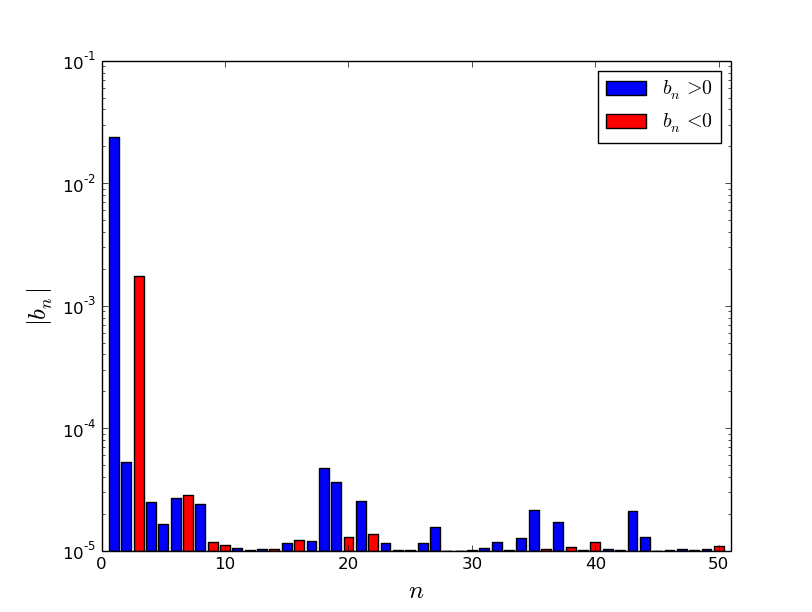
\includegraphics[width=0.95\linewidth] {12.png}
	\caption{Коэффициенты для приближенного решения (\ref{26}) --- несимметричное возмущение.}
	\label{fig:12}
  \end{center}
\end{figure} 

\begin{figure}[!h]
  \begin{center}
\begin{minipage}{0.051\linewidth}
\center{1} \\
\end{minipage}
\hfill
\begin{minipage}{0.3\linewidth}
\center{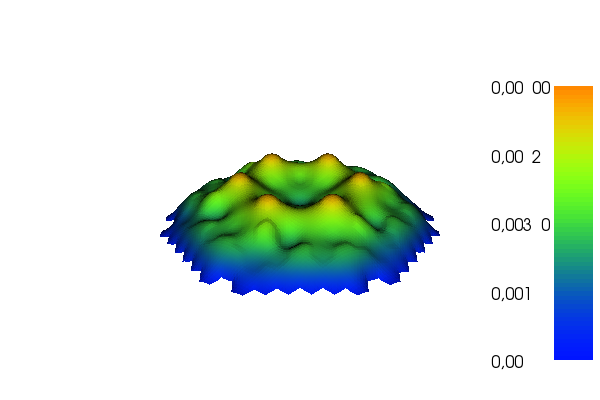
\includegraphics[width=1\linewidth]{13-11.png}} \\
\end{minipage}
\hfill
\begin{minipage}{0.3\linewidth}
\center{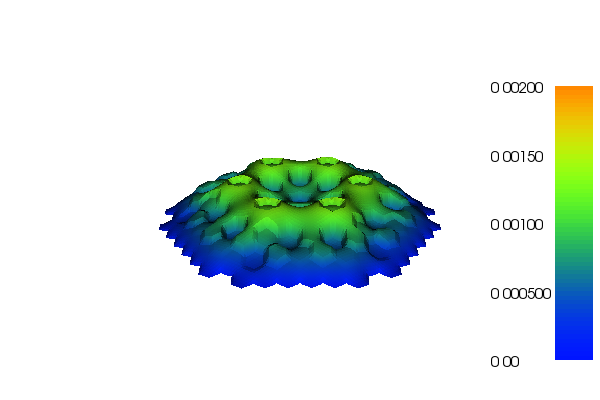
\includegraphics[width=1\linewidth]{13-12.png}} \\
\end{minipage}
\hfill
\begin{minipage}{0.3\linewidth}
\center{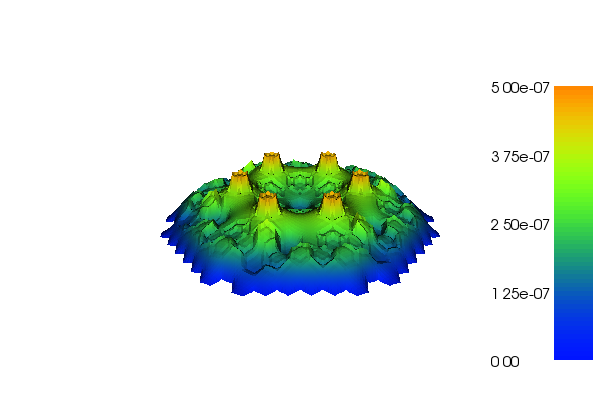
\includegraphics[width=1\linewidth]{13-13.png}} \\
\end{minipage}

\begin{minipage}{0.051\linewidth}
\center{2} \\
\end{minipage}
\hfill
\begin{minipage}{0.3\linewidth}
\center{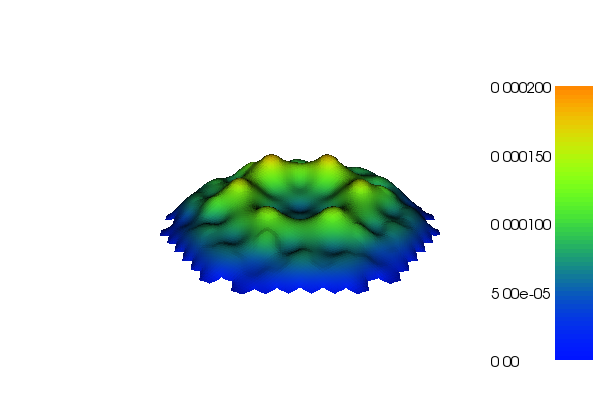
\includegraphics[width=1\linewidth]{13-21.png}} \\
\end{minipage}
\hfill
\begin{minipage}{0.3\linewidth}
\center{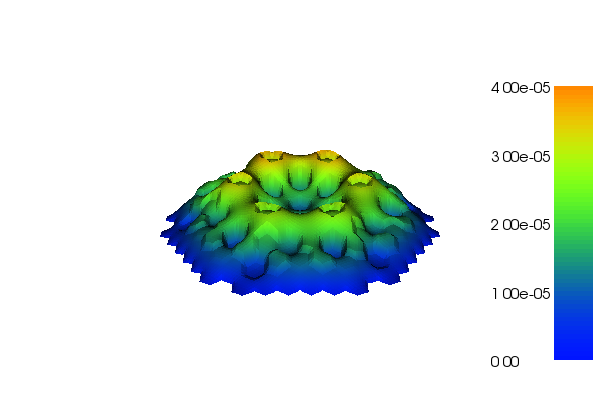
\includegraphics[width=1\linewidth]{13-22.png}} \\
\end{minipage}
\hfill
\begin{minipage}{0.3\linewidth}
\center{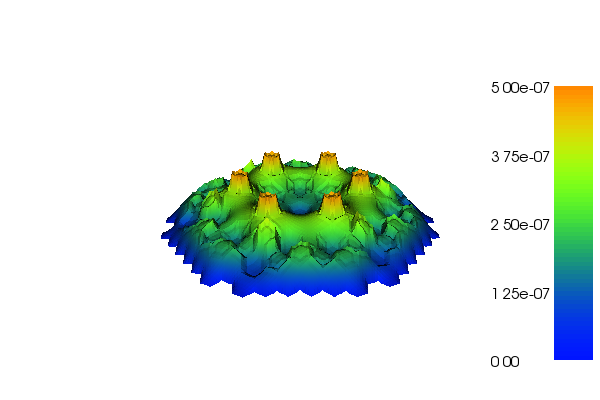
\includegraphics[width=1\linewidth]{13-23.png}} \\
\end{minipage}

\begin{minipage}{0.051\linewidth}
\center{ } \\
\end{minipage}
\hfill
\begin{minipage}{0.3\linewidth}
\center{a} \\
\end{minipage}
\hfill
\begin{minipage}{0.3\linewidth}
\center{b} \\
\end{minipage}
\hfill
\begin{minipage}{0.3\linewidth}
\center{c} \\
\end{minipage}
\hfill

\caption{Функция $\bm u(\bm x, 0)$ (строка 1) и функция  $\bm u_N(\bm x, 0)$ (строка 2) для несимметричного возмущения:
a --- neutron flux of 1 group, b --- neutron flux of 2 group, c --- delayed neutron.}
\label{fig:13}
  \end{center}
\end{figure}

\subsection{Сравнение с решением нестационарной задачи} 

Приближенное решение, которое получено на основе modal approximation,
можно сравнить с решением динамической задачи.
Решается краевая задача для системы уравнений (\ref{22}).
Используется (смотри детали в \cite{nd-mm}) полностью неявная схема
на равномерной сетке по времени с достаточно малым шагом $\tau = 0.0025$.
Динамика neutronic power ядерного реактора $P$ и запаздывающих нейтронов $C$ 
на начальной стадии при переходе от накритического состояния в подкритическое при
симметричном возмущении показана рис.\ref{fig:14}. 
Здесь 
\[
 P(t) = \int_{\Omega} (\nu\Sigma_{f1} \varphi_1 + \nu\Sigma_{f2} \varphi_2)  d \bm x,
 \quad C(t) = \int_{\Omega} c(\bm x,t) d \bm x.
\] 
Наблюдается быстрое изменение neutronic power на небольшом отрезке времени, 
при этом запаздывающие нейтроны перестаиваются слабо.
Динамика медленной фазы иллюстрируется рис.\ref{fig:15}, \ref{fig:16}. 
Здесь приведены как решения, полученные при использовании полных уравнений (dynamic на рис.\ref{fig:15}, \ref{fig:16}),
так и решение при использовании modal approximation (modal).
Аналогичные данные для несимметричного возмущения накритического состояния реактора приведены
 рис.\ref{fig:17}, \ref{fig:18}. 
Мы видим, что с хорошей точностью передаются интегральные характеристики динамики реактора
на медленной стадии.

\begin{figure}[!h]
  \begin{center}
    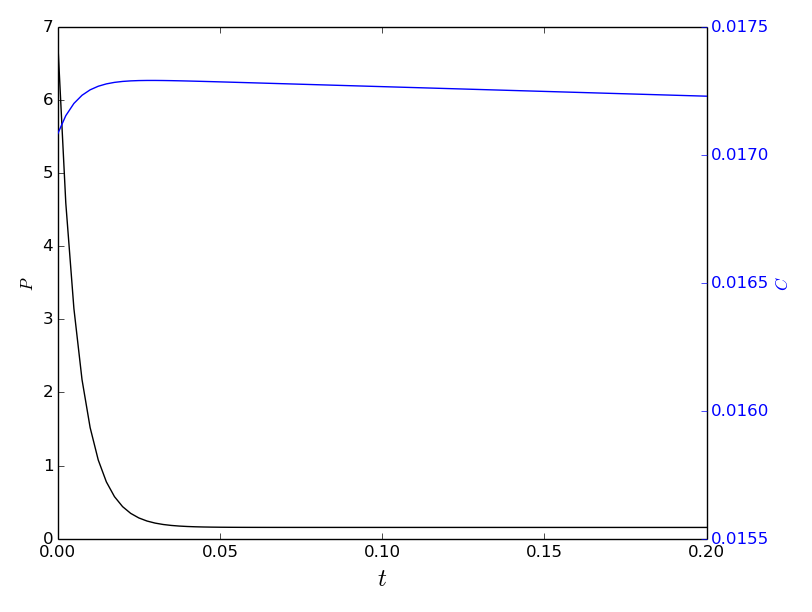
\includegraphics[width=0.9\linewidth] {14.png}
	\caption{Быстрая фаза изменения состояния.}
	\label{fig:14}
  \end{center}
\end{figure} 

\begin{figure}[!h]
  \begin{center}
    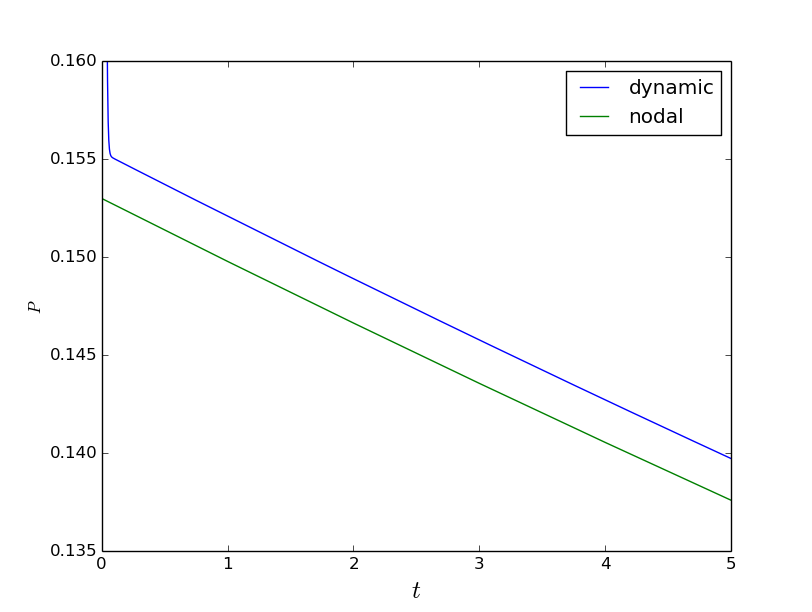
\includegraphics[width=0.9\linewidth] {15.png}
	\caption{Медленная фаза изменения состояния: neutronic power}
	\label{fig:15}
  \end{center}
\end{figure} 

\begin{figure}[!h]
  \begin{center}
    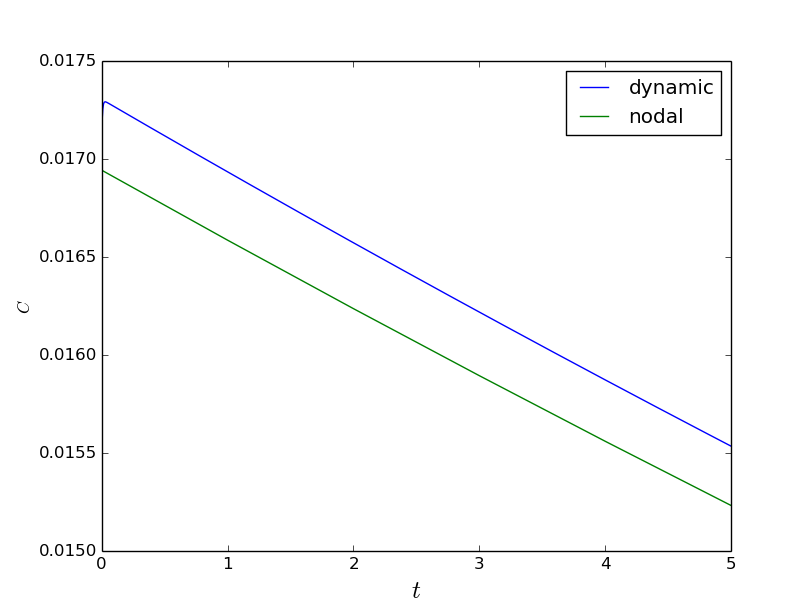
\includegraphics[width=0.9\linewidth] {16.png}
	\caption{Медленная фаза изменения состояния: запаздывающие нейтроны}
	\label{fig:16}
  \end{center}
\end{figure} 

\begin{figure}[!h]
  \begin{center}
    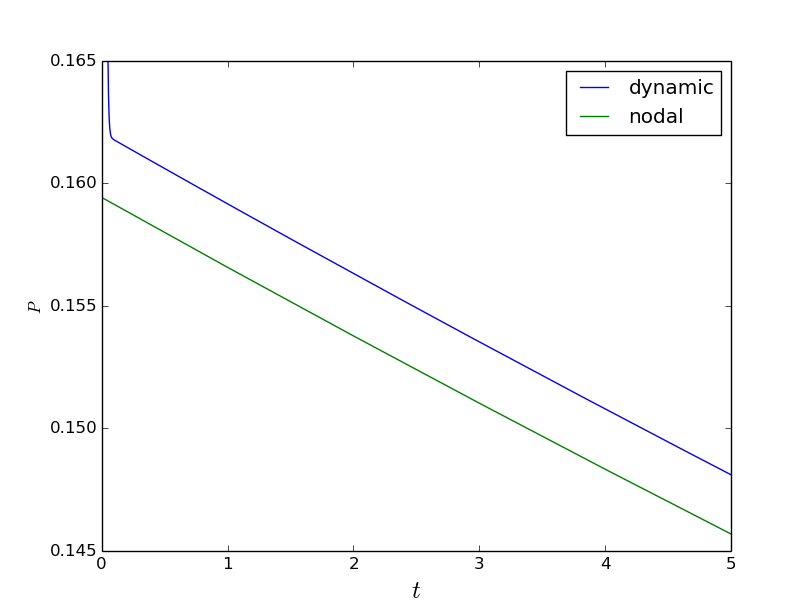
\includegraphics[width=0.9\linewidth] {17.png}
	\caption{Медленная фаза изменения состояния при несимметричном возмущении: neutronic power}
	\label{fig:17}
  \end{center}
\end{figure} 

\begin{figure}[!h]
  \begin{center}
    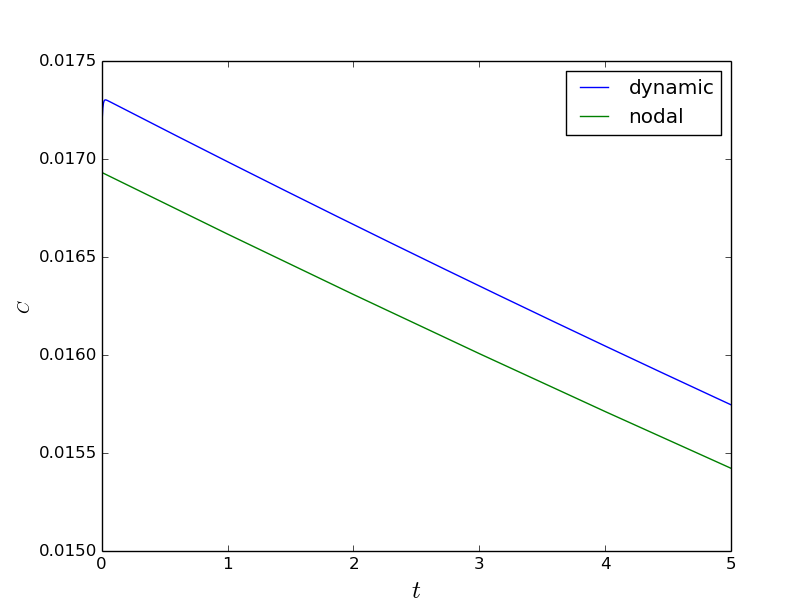
\includegraphics[width=0.9\linewidth] {18.png}
	\caption{Медленная фаза изменения состояния при несимметричном возмущении: запаздывающие нейтроны}
	\label{fig:18}
  \end{center}
\end{figure} 

\clearpage


\section{Conclusions} 

Рассматривается проблема моделирования динамических процессов в ядерном реакторе на основе
многогрупповых уравнений диффузии нейтронов с учетом запаздывающих нейтронов.
Используется modal approximation, когда приближенное решение раскладывается
по небольшому набору dominant собственных функций  $\alpha$-eigenvalue спектральной задачи.

Численное моделирование нестационарных
процессов в ядерном реакторе проводиться на основе последовательной смены состояний 
реактора, которые характеризуются набором постоянных многогруппового описания нетронного поля.
В разработанном state change modal method выделяется
фаза быстрого перехода к приближенному решению в виде набора доминантных мод.
На медленной фазе динамики реактора решение строиться на основе эволюции
dominant мод.

Вычислительная реализация state change modal method базируется на основе
предварительно рассчитанных (of-line calculation) собственных значениях 
и собственных функций  $\alpha$-eigenvalue спектральной задачи.
Быстрое выделение dominant мод и расчет нейтронного поля реактора на отдельные моменты времени
проводиться на основе on-line calculation.

Для аппроксимации по пространству используются классические  Lagrange finite elements степени  $p=1,2,3$. 
Контроль точности проводиться на основе сгущения сеток. 
Спектральные задачи численно решаются с использованием хорошо разработанного свободного
программного обеспечения SLEPc.

Test calculations are made in two-dimensional approximation for a model of VVER-1000 reactor without reflector 
using two-group diffusion approximation. Выполнены расчеты доминантных мод 
для ядерного реактора в надкритическом состоянии. 
Решение с главной модой, которое определяет регулярный режим реактора, используется 
как начальное условие для перехода в подкритический режим. 
Проведено моделирование смены динамики перевода реактора в новое состояние
в двух вариантах. Первый из них (симметричное возмущение) соответствует 
одинаковому изменению свойств поглощающего материала.
Второй вариант  (несимметричное возмущение) связан с разным изменением свойств поглощающего материала
по половинам сечения активной зоны реактора.

Сравнение расчетов на основе modal approximation с расчетами по полной динамической модели
показывает приемлемую точность вычисления nuclear power и общего
количества запаздывающих нейтронов for a model of VVER-1000.

\section*{Acknowledgements}

This work are supported by the Russian Foundation for Basic Research (\#~16-08-01215) 
and by the grant of the Russian Federation Government (\#~14.Y26.31.0013).

\clearpage

\bibliography{scs}

\end{document}
